\documentclass{ecuthesis}
\usepackage{amsmath, amssymb, amscd}
\usepackage[hyphens]{url}
\usepackage{graphicx}
\usepackage{amsthm}
\usepackage[all]{xy}
\usepackage{multicol}
\usepackage{booktabs}
\usepackage{listings}

\usepackage{bchart}

\makeatletter
\patchcmd{\l@chapter}{#1}{\MakeUppercase{#1}}{}{}
\makeatother

\CompileMatrices

\renewcommand\floatpagefraction{.9}
\renewcommand\topfraction{.9}
\renewcommand\bottomfraction{.9}
\renewcommand\textfraction{.1}
\setcounter{totalnumber}{50}
\setcounter{topnumber}{50}
\setcounter{bottomnumber}{50}

\newtheorem{thm}{Theorem}[section] 
\newtheorem{cor}[thm]{Corollary}
\newtheorem{lem}[thm]{Lemma}

\newcommand{\degrees}[0]{\ensuremath{^\circ}}
\newcommand{\dgd}[0]{Directional Graph Drawing}

\title{App Developmentment for Learning Algebra}
\author{Susan Lauer}
\department{Computer Science}
\degree{Master of Science}
\program{Software Engineering}
\date{April 21, 2017}

\advisor{Mark Hills, PhD}
\member{Member 2, PhD}
\member{Member 3, PhD}
\departmentchair{Venkat Gudivada, PhD}
\dean{Paul J. Gemperline, PhD}

\thesismonth{April}
\thesisyear{2017}

\begin{document}


\begin{abstract}
\noindent Powered by increased capabilities of online collaboration tools, open source software development has become a critical component of the development landscape for both individual developers and for organizations. However, very little is known about how developers and organizations in regions with a heavy information technology presence participate in the open source community. This research uses public data from GitHub, a popular online open source collaboration tool, to gain a better understanding of open source software development activity in one such region, the Research Triangle Park in North Carolina. Research Triangle Park is one of the largest research parks in the world, and the largest in the United States. Within the 7,000 acre park, there are currently more than 200 companies employing around 50,000 people in a number of fields of expertise, with information technology playing a large role. To explore how developers and organizations in this region are involved in open source development, we use data mined from GitHub to aggregate information and trends about the developers and organizations themselves, their open source projects, and their use of the social media features within GitHub. The data collection tools and techniques created to enable this research are designed to easily enable similar studies to be performed for other geographical regions.
\end{abstract}

\coversheet

\maketitle
\makecopyright
\makesignature
\tableofcontents
\listoftables
\listoffigures

\chapters

% !TEX root = main.tex
\chapter{Introduction}
\label{Chapter:Introduction}

Open source software development is continuing to grow within information technology communities. The data capable of being extracted from collaborative development platforms gives researchers an opportunity to answer many questions about open source project activity and trends. However, at this point in time, we know little about how people are participating in open source development from a regional perspective. This research is aimed at studying open source activities through public data within GitHub \cite{_github_2016} to understand what the open source software engineering demographic looks like in Research Triangle Park (RTP), NC, one of the most prominent research parks in the world. 

GitHub is a widely used platform for open source software development and collaboration. Its extensive features give software developers the capability to join forces with others from all over the world on a variety of projects, from small projects to major projects that are being used at the enterprise level. GitHub provides a public REST API which grants researchers the opportunity to mine and study this data from an empirical perspective. Using the GHTorrent Project \cite{gousios_ghtorrent:_2012}, \cite{gousios_ghtorent_2013} as our foundation for information, we focus on answering a few key questions throughout this research:
\begin{enumerate}
\item What do the metrics look like around individual users and organizations and their involvement in open source projects in the RTP area? 
\item What do the overall numbers look like with regards to projects being developed by users and organizations in the RTP region? How active are these projects, and are they still relevant since inception?  
\item How do users and organizations in the RTP region use the social media features available on GitHub?
\end{enumerate}

While the answers to these questions have focused on the RTP region, the scripts developed for this empirical study can also, with some generalization, be used to study other geographic areas, which will enable future research including answering similar questions for other regions and comparing multiple regions. Chapter 2 will go through key reasons on why RTP was chosen as a strategic location for this research. Chapter 3 will provide more information around GitHub, with an overview of terms and associated workflows, as well as an overview of the GHTorrent project. Chapter 4 will discuss related research on this topic, particularly studies into open source data. Chapter 5 and 6 will go through the methodologies used for data collection and then provide analysis of the RTP data collected. Lastly, we will wrap up in Chapter 7 with closing remarks about this research and ideas for future research. 

\paragraph{Research Contribution:} Through empirical techniques applied to data mined from project repositories on GitHub, this thesis quantitatively shows how both individual developers and organizations participate in open source software development in the Research Triangle Park region of North Carolina. The process used to extract and compute over the repository data has been scripted to ensure the reported results can be easily replicated, while the scripts themselves have been designed to enable future studies of other technology regions as well as comparative studies of multiple regions. The data collection tools and techniques created to enable this research are publicly available on GitHub (User ID: LindseyKLanier, \cite{_lindsey_github}) under an open-source license. 
% !TEX root = main.tex
\chapter{Overview of Research Triangle Park}
\label{Chapter:RTP}

In this chapter, we first define Research Triangle Park, the region studied in this thesis. We then explain why this region was chosen for this study, focusing on the rapid growth of the region and the significant presence of high tech companies and major universities.

\section{Where is Research Triangle Park?}
Research Triangle Park (RTP) is the largest research and science park in North America, and one of the largest in the world. The park, which stretches 7,000 acres across Wake and Durham counties was founded in 1959 by the Research Triangle Foundation. RTP is not a city, but it has its own special county district \cite{_research_????}. The Research Triangle Region Organization, a partnership dedicated to overseeing collaboration between businesses, government and various other institutions within the region identifies RTP as the following counties (see Figure \ref{fig:rtp-region}): Chatham, Durham, Edgecombe, Franklin, Granville, Harnett, Johnston, Lee, Moore, Nash, Orange, Person, Vance, Wake, Warren, and Wilson \cite{_research_????}. Additionally, the RTP Organization has stated that the RTP metro area has a population of 1.3 million people, and that there are 3 million people within a 60-mile radius of the park \cite{weddle_research_????}. Our project utilized public NC League of Municipalities (NCLM) data to identify all of the cities in each of the RTP counties to assist our research \cite{_north_????}.

\begin{figure}
\begin{center}
\resizebox{\textwidth}{!}{
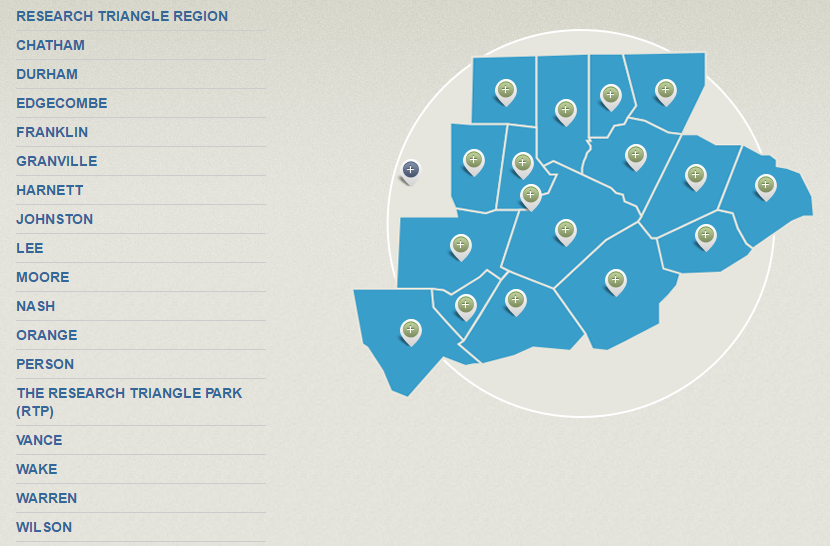
\includegraphics{Images/RTP-Region_2.png}
}
\caption{RTP region as defined by Research Triangle Region Organization \cite{_research_????}}
\label{fig:rtp-region}
\end{center}
\end{figure}

\section{Why Research Triangle Park?}

Many reasons can be attributed to our choosing of RTP and its surrounding communities for initial research into local open source activities. Over the last decade, numerous media outlets and journalists have continuously given this region nicknames such as “Start-up Capital of the South” \cite{_durhams_????} and “The Next Silicon Valley” \cite{_4_????}. Between 2000 and 2012, Raleigh's population grew 47.8 percent, which topped Forbes's list of fastest growing metropolitan areas in the country. This number was more than three times the overall growth of all other metropolitan areas \cite{kotkin_americas_????}. The Google for Entrepreneurs Network has invested in 3 different locations in Raleigh/Durham (RDU) for what they call "American Underground". American Underground is referred to as a "Start-Up Incubator" where software groups can rent space for their teams to meet and work \cite{_american_????}. The Research Triangle Park Organization continues to drive their mission to "change the course of history" by bringing people together and fostering innovation and creativity in the RTP community \cite{_research_2016}. They've recently open up a new center, The Frontier, with free space for teams to collaborate and participate in a variety of networking events \cite{_frontier_????}. 

Outside of the start-up communities, many big technology players have a presence in RTP--Red Hat, Citrix, Cisco, NetApp, IBM, Microsoft, Google, SAS, and others,  with more news about others following every year. There are several local prestigious universities including the University of North Carolina Chapel Hill, North Carolina State University, and Duke University, all of which are consistently producing top talent within the science, math and technology industries. According to the Research Triangle Park Organization \cite{_research_2016}, local companies and organizations have won Nobel Prizes and the Pulitzer. To date, they've recorded that there have been 245 company start-ups, 3,256 patents, and 1,970 trademarks. 

At the beginning of 2016, the North Carolina State of Technology Industry Report was released. We found some of the statistics produced by this group (NC Technology Association and Economic Leadership of Raleigh) relevant to reasons we chose the RTP region, even though they were specific to the state as a whole \cite{_nc_????}. 

A few of the highlights from this report included:

\begin{itemize}  
\item North Carolina is the \#2 state in Information Technology (IT) employment growth from 2009-2014.
\item North Carolina is the \#4 state for University Technology Licenses and Options Executed with 242 licenses and options in 2014.
\item Future North Carolina tech sector growth is expected to outpace national and American South averages.
\item Over the past year technology employment grew by 3.6 percent, and technology establishments grew by 5.2 percent.
\end{itemize}

These statistics can serve as a proxy for choosing to do research on other areas with a large and growing presence in the information technology industry.

% !TEX root = main.tex
\chapter{GitHub and The GHTorrent Project}
\label{Chapter:Background}

In this chapter, we will give an overview of GitHub as a platform as well as the GHTorrent project and it's associated data source. GitHub and GHTorrent provide data which is the foundation to the research performed in this thesis.

\section{GitHub}
\label{sec-GitHub}
GitHub is a web-based platform used for version control and collaboration between developers. Users can choose to utilize standard Git commands in a terminal to manage their code on GitHub or use the GitHub graphical user interface (GUI) and associated features on GitHub.com. As of February 2016, there were 12 million people collaborating across 31 million repositories on GitHub \cite{_github_2016}. Users wanting to create a GitHub account for their projects have two options, public (free) and private (paid). Public repositories are heavily used by open-source teams to allow for code storage and collaboration from users all over the world. GitHub gives users the option to create "organizations" to more easily manage teams. Organizations allow teams to group one or more projects under one umbrella. Multiple owners can be mapped to organizations for settings and permissions management. 

This research pulls data on GitHub's source code management features with a focus on mining RTP specific statistics as well as looking into the involvement that RTP users have in the social networking aspect of the platform. Source code packages hosted on GitHub are referred to as repositories. We utilize the GHTorrent Project \cite{gousios_ghtorent_2013} for data collection of RTP specific (public) repositories. Public repositories can be browsed and contributed to by not only the owner but anyone else interested in downloading a local copy. Changes by GitHub users can be submitted to the repository owner for review in the form of a "pull request". Changes are saved to repositories through what are known as "commits". There are various workflows that could be implemented for GitHub projects. One popular option is to utilize "forking" and "pull requests". A "fork" is a clone of a repository, saved as a new repository on one's own GitHub account. Users might implement their own enhancement to the cloned application, or could also work on an associated "issue". One or more commits can be pushed to this clone. Once the developer is finished with their changes, they can then submit a "pull request" to the original repository owner for review. If the repository owner is happy with the changes, they can merge the "pull request" into a branch on the original repository. This is the main workflow that we focus on throughout this research.

During the data collection phase of this research, we noted some important details about commits which were unexpected. The author for any given commit is the user who wrote the code to be committed, the committer is the user who pushed this code into the main software repository. Git allows users to commit on behalf of another person, hence the commit can be pushed by someone who did not author it. Depending on the workflow used to commit the code change, the author/committer information can vary. For example, if a user commits a code change through the command line on their local machine they can include author and committer information as free text form (not ideal if they spell their e-mail address wrong). GitHub has a large knowledge base which documents its various features, including a help article which explains this commit information further \cite{_why_????}.

There are also many useful social networking features available on GitHub. GitHub allows users to follow friends and track what they are working on. Users can also follow particular repositories and see associated updates, also known as "stargazing". GitHub also provides an interface which shows which repositories are trending at any given time, and which can be sorted by programming language.

\section{The GHTorrent Project}
\label{sec-GHTorrentProject}
GHTorrent was created for the software research community, a place to easily come to query specific sets of open source repository data without having to go through the GitHub REST API directly. GHTorrent has a relational database (MySQL) which stores structured data on users, repositories, commits, etc. GHTorrent stores the bulk of its data in a MongoDB instance. MongoDB is a type of NoSQL database which utlizes JSON and allows for rapid changes and agile development. MongoDB stores data in the form of JSON documents within what they call "collections". Collections can compare slightly to a relational database's "table" but they are quite different themselves in that they are dynamic, flexible and do not need to have a defined schema. The collections included in GHTorrent's MongoDB instance are outlined in Table \ref{fig:ghtorrent-collections}. MongoDB provides advanced querying operations such as Map-Reduce and aggregation which gives data miners flexibility when conducting their research \cite{_mongodb_????}. GHTorrent chose this technology to be able to more easily manage the large collections of dynamic data as well as accommodate changes to the GitHub schema quickly, among other reasons such as giving the research community flexible options for querying \cite{gousios_ghtorrent:_2012}. 

\begin{table}
\centering
\begin{tabular}{|c|c|}
\hline
\textbf{Collection name} & \textbf{Github API URL} \\
\hline
commit\textunderscore comments & \#{user}/\#{repo}/commits/\#{sha}/comments \\
\hline
commits & repos/\#{user}/\#{repo}/commits \\
\hline
events & events \\
\hline
followers & users/\#{user}/followers \\	
\hline
forks & repos/\#{user}/\#{repo}/forks \\	
\hline
issues & /repos/\#{owner}/\#{repo}/issues \\	
\hline
issue\textunderscore comments & repos/\#{owner}/\#{repo}/issues/comments/\#{comment\textunderscore id} \\
\hline
issue\textunderscore events & repos/\#{owner}/\#{repo}/issues/events/\#{event\textunderscore id} \\
\hline
org\textunderscore members & orgs/\#{org}/members \\
\hline
pull\textunderscore request\textunderscore comments & repos/\#{owner}/\#{repo}/pulls/\#{pullreq\textunderscore id}/comments \\
\hline
pull\textunderscore requests & repos/\#{user}/\#{repo}/pulls \\	
\hline
repo\textunderscore collaborators & repos/\#{user}/\#{repo}/collaborators \\ 
\hline
repo\textunderscore labels & repos/\#{owner}/\#{repo}/issues/\#{issue\textunderscore id}/labels \\
\hline
repos & repos/\#{user}/\#{repo} \\
\hline
users & users/\#{user} \\
\hline
watchers & repos/\#{user}/\#{repo}/stargazers \\
\hline
\end{tabular}
\caption{List of collections available in the GHTorrent MongoDB instance.}
\label{fig:ghtorrent-collections}
\end{table}

The GHTorrent project included 4TB of data in their MongoDB instance (as of January 2015) \cite{gousios_ghtorent_2013} but according to more recent updates on their Twitter feed \cite{_ghtorrent_????} (@ghtorrent), it has been constantly growing and aims to pull not only more recent data but to store the entire historical GitHub data source. Their Twitter feed  (@ghtorrent) keeps the community up to date with regular posts, most recently noting that Microsoft has agreed to sponsor the project on Azure for the next 2 years. GHTorrent's users collection was recently geocoded using OpenStreetMap (OSM) data and interestingly, the code for geocoding was provided by a local RTP contributor (GitHub Login: DerekTBrown). This particular feature was extremely helpful for our research in that we could query users based off their geocoded city or state instead of parsing the free text location field ourselves.

As documented in \cite{gousios_ghtorrent:_2012} – which was written during the initial stages of GHTorrent's development (2012), there are several challenges that researchers would face if they decided to use the GitHub REST API directly, challenges that the GHTorrent project has overcome through their provided data source. One of the main challenges is that the GitHub data source is massive. Unless you know exactly what you are looking for and where to look for it, it may take days to search through the collections given the 5000 request/hour limit per API key. The GHTorrent project has done the heavy lifting for us by reverse engineering and documenting the GitHub schema and REST API. Having that information readily available saves researchers much time from having to do this themselves.

In order to overcome the 5000 request/hour limit per API key, GHTorrent designed their workflow to be distributed, with the research community donating SSH keys to allow for extra workers and concurrency across a cluster of machines. SSH keys can be donated by members of the GitHub community \footnote{We donated SSH keys to enable this.}.  GHTorrent uses the REST API \cite{_github_????} (Events Stream) to collect static repository information as well as other events such as associating commits with users and repositories. They have a messaging layer (RabbitMQ) which sits between the events stream and aids with pushing out further requests to the API from there. A single event can ultimately lead to many downstream requests to gather more information from other parts of the REST API. GitHub's event stream is constantly flowing with new information as users are working inside projects. For example, each commit fires off a number of creation requests to other parts of the overall schema. A documented limitation for this is that the event stream handles all additive actions but does not report deletions.  \cite{gousios_ghtorent_2013}

As with all large scale projects, there are challenges and limitations documented for GHTorrent. As highlighted in the previous section, it is possible for the author and the committer to be two different people and there can sometimes be issues with the mapped user credentials when commits are pushed via the command line (free text is allowed). If GHTorrent is unable to map the user to a commit, it creates a fake user entry until the next request is created when it will attempt to resolve the fake entry. As of 2013, there were several thousand fake users in the data source. Another potential problem with the quality of the data is staying on track of any regular updates to the GitHub schema itself. As GitHub makes changes to its overall schema, the GHTorrent project has to closely monitor in case any changes are required to its processes. Another potential problem with the quality of this data source is that there are known periods of missing data from the event stream due to an error in a couple of the GHTorrent scripts---these periods include a few days in March 2012 and mid-October through mid-November 2012. \cite{gousios_ghtorent_2013} 
% !TEX root = main.tex
\chapter{Related Work}
\label{Chapter:RelatedWork}

There have been a large number of studies done on open source software, particularly the mining of GitHub data to gain a better understanding of how the widely popular tool is being used across the globe. Due to the incredibly large nature of GitHub as a platform (as highlighted in Chapter \ref{Chapter:Background}), it is important for researchers to understand first the questions they want to answer and second the various options they have available to collect GitHub data prior to starting the mining process. Cosentino, Luis and Cabot collected 231 works on mining GitHub, eventually narrowing these down to a set of 93 which they use to try and better understand how GitHub repositories are being mined, how the data ends up being used and how associated limitations are presented and addressed \cite{cabot_should_2016}. They discuss overall limitations with the use of various GitHub datasets and the fact that they are not always current or consistent. They also found that two thirds of the 93 selected works did not provide enough information for future comparative studies to replicate the work. They discuss limitations of their own study and conclude by highly suggesting that researchers ensure datasets and instructions to replicate studies on mining GitHub are shared with the research community. 

Prior to beginning this research on the RTP area, ideas on what we wanted to focus on were formed through the perusal of various published papers. Related work on topics such as the impact of geography on contributions in GitHub, determination of local skill sets based off GitHub data, programming language trends, the impact social networking features have on users as well as a study that looked to determine the promises and perils of mining GitHub through user surveys will be cited and discussed further in this chapter. The most important piece of research that we initially focused on was the GHTorrent project created by G. Gousios. Much of the information sourced from this project's public research is already outlined in Chapter \ref{Chapter:Background}. We were able to use the GHTorrent data source as a means to quickly get started in searching for RTP specific data on users, their repositories and overall open source activity, which we later use to answer questions on what the social engineering demographic looks like in RTP.

A study was done by a group of researchers (including Gousios from GHTorrent) on the “promises and perils” of mining GitHub \cite{kalliamvakou_promises_2014}. At that point, there were no known studies of the quality and properties of data available through GitHub. This research was focused around trying to gain a better understanding of how users take advantage of the various capabilities that they are exposed to within GitHub, particularly committing, submitting pull requests and issues. Out of the 1,000 surveys sent to active users who had listed their e-mail address on their GitHub account, only 240 responses came back. Although the sample was small, the researchers were able to collect some valuable information which they share as part of their research. This study concluded, in summary, by showing that most repositories are inactive and only created for personal reasons. We can conclude similar results as part of our research on the RTP area given the number of repositories that were created and never touched again. These researchers also found out through a survey, that many developers host their code on GitHub for the sole reason of free hosting, having no desire to ever open it up for collaboration. In addition, 38\% of users involved in the survey said they use GitHub primarily for their own projects, with no intention of collaboration with other developers. Due to these findings, the authors provide recommendations based on their research to suggest the best way to study GitHub data as a whole by explaining in detail some of the different workflow use cases that they are aware of for personal and project work. 

In today's communities (from our experience), development of software is quite often split between different regional teams. As audio/video collaboration technologies continue to advance, the distance of these teams matter less. However, there are still many instances where regional clusters contain concentrated software engineering industries---RTP being an example as we are demonstrating through this research. Takhteyev and Hilts did research on the geography of open source software through GitHub \cite{takhteyev_investigating_2010}. These researchers came up with a unique method to study regional teams and their associated involvement in open source projects. They started with a single account (one of GitHub's founders) and began collecting more accounts and information based off of their connections, ending up with a sample of 70,414 accounts. As we mentioned previously, the location field in a GitHub user's public profile is free text and hence difficult to query directly. This team created a method to code the location using Geonames.org, Yahoo's GeoAPI, as well as some manual intervention. They were able to conclude (based on sample accounts) that 39\% of all GitHub accounts are located in the United States, the remaining 61\% being spread across the globe (second largest country being the United Kingdom at 7\%). The top 5 clusters identified in the United States were San Francisco, New York, Boston, Seattle, and Chicago.

David Rusk and Yvonne Coady from the University of Victoria did some research on analyzing the popularity of programming languages in their local community (Victoria, BC, Canada) in 2014 \cite{rusk_location-based_2014}. One of the goals to this research was to give employers as well as potential employees a better idea of what the local skill sets look like through a talent pool repository as well as an overview of the common technologies used in any given location. This team created a tool which pulled data out of the GitHub REST API and dumped it into a MongoDB instance. It is unclear why they did not use the GHTorrent data source as it was cited as related work and all of this information could have been pulled directly from the GHTorrent MySQL instance itself. They were able to create some visualizations similar to what was done during the data analysis phase of this project and provided these to local developers and businesses for feedback. They discussed that most of the developers found the information quite helpful, some being a bit concerned with developer privacy given the researchers were publishing names and other bits of personal information within the project itself. Others pushed back and highlighted the fact that these profiles were already public to begin with and that listing them within the project was a required feature. Employer feedback was also positive, they were happy with the fact that they could find developers with specific skills, code samples they've written, as well as contact information all in one place. Their aim was to be able to expand this to other locations as part of future work. As our research looks at similar metrics for the RTP region, publishing this data could prove useful in the future. 

In 2013, Begel, Bosch and Storey conducted interviews with 4 leaders from the software development industry to try and gain a better understanding around the social networking aspects of open source software development \cite{begel_social_2013}. Brian Doll, an engineer in the marketing space for GitHub was interviewed as part of this initiative. We found some of his answers particularly interesting and could relate them back to some of the questions we were looking to answer as part of this research. Storey asked Doll, "How does social networking play a role in the services you provide?" Doll then started describing a recent e-mail he had received from a past colleague who had mentioned he was following his activity on GitHub, such as the repositories he had starred. In this way, users are able to keep up with various projects that their connections are watching or actively participating in. We explain how often RTP users are utilizing this feature as part of our local research. Doll was also asked how other relationships were formed on GitHub, outside of the “stargazing” technique. He started describing some of the use cases for creating a GitHub “organization” user type – which is something we look at the usage of for our local research. Doll mentions that it is quite common for projects to be managed in this way on GitHub because "it's the cleanest way for them to give permissions to several developers with different levels of access to the code." Another important point that Doll makes in this interview is the importance that GitHub sees in ensuring users can “put a face to the name of the project's main developer.” This way, the user who is doing the bulk of the work is getting the actual credit for it. For this reason, GitHub keeps the user login ID in the URL structure of each repository, and also makes heavy use of avatars in activity feeds. This point is interestingly related to the current controversy over privacy between GHTorrent project and GitHub users \cite{_issue_????}. Doll also discusses his opinion around the benefit of open source software development for people looking to get a job within a programming company, regardless of experience, and discusses articles that he has read which claim GitHub as being “the new resume for programmers”. 

% !TEX root = main.tex
\chapter{Data Collection}
\label{Chapter:Collection}

This chapter will walk through the data collection method that was developed for this thesis. The GHTorrent project was chosen as our main source to collect GitHub data on local projects in order to gain a better understanding of what the local open source community looks like in RTP. The ultimate goal of this research was to not only study our region, but to also develop a method that could be reused for future research on other locations through the consolidation of Python and SQL scripts that were created. As explained in Chapter \ref{Chapter:Background}, the GHTorrent project offered an offline mirror of public data pulled from the GitHub REST API and allowed us to get started on our investigations immediately. GHTorrent provides two methods to collect data, a MySQL instance which includes structured meta-data and a MongoDB instance which includes in-depth GitHub information in the form of JSON documents. An example of a query and associated results from both MySQL and MongoDB can be found in Figure \ref{fig:example-MySQL} and Figure \ref{fig:example-MongoDB} respectively. These figures give an idea of how much more information is stored in the GHTorrent MongoDB versus MySQL instance.

\begin{figure}
\footnotesize
\begin{lstlisting}
MySQL Query:
select id, login, name, location 
	from users 
	where login = 'lindseylanier'

Results:
\end{lstlisting}
\centering
\footnotesize
\begin{tabular}{|c|c|c|c|}
\hline
id & login & name & location \\
\hline
5641774 & lindseylanier & Lindsey Lanier & USR \\
\hline
\end{tabular}

\caption{Example of a MySQL query to pull the information on one user and the associated results after executing.}
\label{fig:example-MySQL}
\end{figure}


\begin{figure}
\tiny
\begin{lstlisting}
MongoDB Query:
> db.users.find({"login":"lindseylanier"}).pretty()

Results:
{
        "_id" : ObjectId("56c563256480fd331e002493"),
        "login" : "lindseylanier",
        "id" : 8949639,
        "avatar_url" : "https://avatars.githubusercontent.com/u/8949639?v=3",
        "gravatar_id" : "",
        "url" : "https://api.github.com/users/lindseylanier",
        "html_url" : "https://github.com/lindseylanier",
        "followers_url" : "https://api.github.com/users/lindseylanier/followers",
        "following_url" : "https://api.github.com/users/lindseylanier/following{/other_user}",
        "gists_url" : "https://api.github.com/users/lindseylanier/gists{/gist_id}",
        "starred_url" : "https://api.github.com/users/lindseylanier/starred{/owner}{/repo}",
        "subscriptions_url" : "https://api.github.com/users/lindseylanier/subscriptions",
        "organizations_url" : "https://api.github.com/users/lindseylanier/orgs",
        "repos_url" : "https://api.github.com/users/lindseylanier/repos",
        "events_url" : "https://api.github.com/users/lindseylanier/events{/privacy}",
        "received_events_url" : "https://api.github.com/users/lindseylanier/received_events",
        "type" : "User",
        "site_admin" : false,
        "name" : null,
        "company" : null,
        "blog" : null,
        "location" : null,
        "email" : null,
        "hireable" : null,
        "bio" : null,
        "public_repos" : 6,
        "public_gists" : 0,
        "followers" : 0,
        "following" : 0,
        "created_at" : "2014-09-28T18:15:42Z",
        "updated_at" : "2016-01-06T02:33:15Z"
}
\end{lstlisting}
\caption{Example of a MongoDB query to pull the information on one user and the associated results after executing.}
\label{fig:example-MongoDB}
\end{figure}

In the beginning of the data collection phase, specific meta-data (which will be discussed further in future sections in this chapter) was pulled on RTP users and repositories by running SQL scripts against the GHTorrent MySQL database. We then used the meta-data collected and queried the GHTorrent MongoDB collections (see Table \ref{fig:ghtorrent-collections} for the full list of available collections) for further information. The meta-data was needed to meet GHTorrent's various index requirements on their MongoDB instance. Due to the massive data source and heavy loads, indexes are required as GHTorrent's MongoDB instance has a 100 second time limit (non-indexed searches easily surpass this). PyMongo \cite{_pymongo_????}, a Python/MongoDB library was used to connect to the GHTorrent MongoDB instance programatically (although connections using a command prompt were also available and used on occasion for searches). The results from the queries executed against the GHTorrent MongoDB instance were stored in a locally created MongoDB instance for analysis. 

Subsequent sections of this chapter will show a common theme around the method we used to both collect and analyze GitHub data in our local MongoDB instance, namely utilizing MongoDB's aggregaton framework \cite{_aggregation_????}. The aggregation framework provides the capability to write queries and perform powerful transformations on collections that surpass the basic MongoDB "find" operation. We will show the ways aggregation was utilized in this project to calculate data points such as the number of original repositories per user, the number of forked repositories per user, the number of pull requests submitted per user, the number of years each user has been a member of GitHub, programming language popularity, etc. Once the data was aggregated (and new collections were formed), we were able to drill into the various bits of information deeper to gain a better understanding of local activity and answer questions about the users and their associated repositories. The basic MongoDB "find" operation was also used in order to search the newly created collections to pull back datasets used to create the various figures presented in this research.

\section{User Information}
\subsection{Collecting RTP Users}
Before starting to look into the Research Triangle Park data, we first had to identify which cities this region consisted of. As discussed in Chapter~\ref{Chapter:RTP}, the Research Triangle Organization \cite{_research_????} identified the RTP region by county and later we found that the NCLM \cite{_north_????} had a list of associated cities per county. There were a total of 90 cities (see Figure~\ref{fig:rtp-cities}) that we were then able to query the GHTorrent MySQL database instance with. This initial step was required as we couldn't directly start using the GHTorrent MongoDB instance due to the users collection having an index requirement on login name (we could not query the GHTorrent MongoDB instance directly on the location field alone without timing out). Additionally, the geocoding of user locations is only available in their MySQL instance. From the GHTorrent MySQL instance, we were able to export the list of users to a comma separated value (CSV) file. We then wrote a Python script which would iterate through the CSV file and query the GHTorrent MongoDB instance for users by their login name, saving the results to a new collection within our local MongoDB instance. This newly formed users collection gave us the beginning of what would later become a 25GB database of RTP GitHub data.

\begin{figure}
\begin{multicols}{4}
\begin{enumerate}
\item Aberdeen
\item Angier
\item Apex
\item Bailey
\item Benson
\item Black Creek
\item Broadway
\item Bunn
\item Butner
\item Cameron
\item Carrboro
\item Carthage
\item Cary
\item Castalia
\item Centerville
\item Chapel Hill
\item Clayton
\item Coats
\item Conetoe
\item Creedmoor
\item Dortches
\item Dunn
\item Durham
\item Elm City
\item Erwin
\item Four Oaks
\item Foxfire Village
\item Franklinton
\item Fuquay-Varina
\item Garner
\item Goldston
\item Henderson
\item Hillsborough
\item Holly Springs
\item Kenly
\item Kittrell
\item Knightdale
\item Leggett
\item Lillington
\item Louisburg
\item Lucama
\item Macclesfield
\item Macon
\item Mebane
\item Micro
\item Middleburg
\item Middlesex
\item Momeyer
\item Morrisville
\item Nashville
\item Norlina
\item Oxford
\item Pine Level
\item Pinebluff
\item Pinehurst
\item Pinetops
\item Pittsboro
\item Princeton
\item Princeville
\item Raleigh
\item Red Oak
\item Robbins
\item Rocky Mount
\item Rolesville
\item Roxboro
\item Sanford
\item Saratoga
\item Selma
\item Sharpsburg
\item Siler City
\item Sims
\item Smithfield
\item Southern Pines
\item Speed
\item Spring Hope
\item Stantonsburg
\item Stem
\item Stovall
\item Tarboro
\item Taylortown
\item Vass
\item Wake Forest
\item Warrenton
\item Wendell
\item Whispering Pines
\item Whitakers
\item Wilson
\item Wilson's Mill
\item Youngsville
\item Zebulon
\end{enumerate}
\end{multicols}
\caption{List of local RTP cities which were collected and used in this research.}
\label{fig:rtp-cities}
\end{figure}

\subsection{Calculating Total Number of Years on GitHub}
One of the questions we sought to answer was the average number of years that local users had been GitHub members. Per Wikipedia, GitHub was founded 8 years ago in February of 2008 \cite{_github_????}. We were interested in understanding if there were any local, active users that had been around since the start. In order to do this, we had to run a few different PyMongo scripts. The first thing that had to occur was the conversion of the "created at" date in the users collection to an "ISODate". The date field that we pulled from GHTorrent's MongoDB instance was not a proper date format. We were not able to run any aggregation functions on the date until it was converted (see Figure~\ref{fig:convert-to-isodate} which shows an example of how easily we are able to do this with Javascript). Next, we used aggregation to get the number of years the user had been a member and projected the output to a new collection (see Figure~\ref{fig:membership-years}). Once this collection was created, we were able to query for users that had been a member for any specified number of years.

\begin{figure}
\begin{lstlisting}
db.githubRTPUsers.find().
	forEach
    (
    	function(element)
        {
        	element.created_at = ISODate(element.created_at);
            	db.githubRTPUsers.save(element);
        }
    )
\end{lstlisting}
\caption{MongoDB function used to convert the created date to a proper ISODate.}
\label{fig:convert-to-isodate}
\end{figure}

\begin{figure}
\begin{lstlisting}
db.githubRTPUsers.aggregate(
[
	{$project: { _id: 0,
    		item: "$login",
   		diff_days:{
        	$divide:
            [{$subtract: [new ISODate(),"$created_at"]}
                	,1000 * 60 * 60 * 24 / 365]}}},
    	{"$out":"calculated_memberForYears"}
])
\end{lstlisting}
\caption{Aggregation in MongoDB used to get the number of years a user has been a member on GitHub. Results are projected to a new collection within our local MongoDB instance.}
\label{fig:membership-years}
\end{figure}

\section{Repository Information}
\subsection{Collecting RTP Repositories}
Once the local users baseline had been established, we began looking into what these users were working on within the open source world of GitHub. The next baseline that we took was user owned GitHub repositories. Again, due to required indexes (repository name and owner login name) in the GHTorrent MongoDB repositories collection, we needed to pull some meta-data out of the GHTorrent MySQL instance before we could query. We used the previous users CSV file to query the GHTorrent MySQL instance (projects table) for everything where the owner's login name was equal to our user's login name. We exported this information to a new CSV, imported it into our local MongoDB instance, and used it to pull more information on user's repositories from GHTorrent's MongoDB into our local MongoDB instance. This new collection gave us pertinent information about local GitHub repositories which we later used to answer our research questions in the data analysis phase. 

As mentioned in the introduction of this chapter, MongoDB provides an aggregation framework which was used to sort through much of this data. Figure~\ref{fig:repo-count-code} shows an example of calculating the total number of repositories by user with the MongoDB aggregation framework (using PyMongo). Here we set up a "pipeline" using the group, sort, project, and out operators. In this particular example, we sought to group the count of repositories by the owner's login name and sort the results in descending order. Each aggregation created a new document that was projected to a new collection in our local MongoDB instance. The results of this aggregation query helped us address questions we had around how many repositories each RTP user had created. As part of this research, we were also interested in understanding which cities in the region had the most repositories. In order to do this, we created a new collection using the same method just described (MongoDB aggregation framework). These results were captured and are discussed in the next chapter on data findings.

\begin{figure}
\begin{lstlisting}
def repo_count_by_user():
    pip = [
        {"$group": {"_id": "$owner.login", "count": {"$sum": 1}}},
        {"$sort": SON([("count", -1), ("_id", -1)])},
        {"$project" : {"_id":1, "count":1}},
        {"$out" : "calculated_repoCountByUser"}
    ]
    userReposCollection.aggregate(pip)
\end{lstlisting}
\caption{Sample Python code which pulls the total repository count per user using PyMongo and the MongoDB Aggregation Framework.}
\label{fig:repo-count-code}
\end{figure}

%\begin{figure}
%\begin{center}
%\resizebox{\textwidth}{!}{
%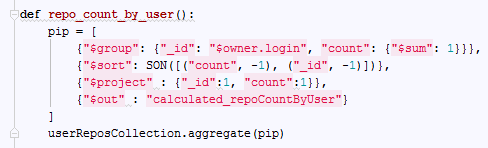
\includegraphics{Images/pymongo-aggregation.PNG}
%}
%\caption{Sample Python code which pulls the total repository count per user using PyMongo and the MongoDB Aggregation Framework.}
%\label{fig:repo-count-code}
%\end{center}
%\end{figure}


\subsection{Original vs. Forked Projects}
\label{origvsforked}
In order to determine original versus forked projects from our collection of local RTP projects, we needed to take a look at the "fork" field for each repository. The "fork" field takes a boolean value of True or False. We wrote a Python function that would count the number of original projects per user as well as the number of forked projects per user. Two separate collections were created in our local MongoDB instance and the data was later analyzed to help us understand if local users were forking existing projects more often than creating new projects.

\section{Overall RTP Activity}
Once we had established a baseline of GitHub users and associated repositories, we could start calculating RTP users' overall activity. As discussed, one piece of this research that particularly interested us was to find out how many users were actually active open source community members, in other words, how many users are actively contributing towards live projects. For this, we wanted to ignore users that joined for one project or homework assignment, for example, and never came back again. 

In order to gain an understanding of the overall GitHub activity in RTP, we investigated from a few different angles. We first aimed to understand trends in overall activity over the lifetime of a local user account and then wanted to understand who is still currently active. We are defining "active" in this research as making a commit to a repository over the last 6 months. In order to determine overall activity, we created the following questions to guide us:

\begin{enumerate}
\item Total number of commits by owner
\item Total number of active repositories based off commits
\item Total number of forks
\item Total number of pull requests
\item Total number of stargazers
\end{enumerate}

Question 1-2 are covered in section \ref{sec-commits}. Question 3 was covered already in section \ref{origvsforked}. Question 4 is covered in section \ref{sec-pullreqs} and question 5 is in section \ref{sec-stargazing}. The results from each data collection method are captured in Chapter \ref{Chapter:Findings}.

\subsection{Collecting User Commits and Active Repositories}
\label{sec-commits}
As part of the study of overall activity within our local scope, we sought to understand what the total number of commits per project looked like. In order to collect this information, we used the meta-data located in the GHTorrent MySQL instance in combination with our already existing collection of local users in our local MongoDB instance. We queried the GHTorrent MySQL instance for the name of the repository, the owner name, the count of commits as well as the last commit date. Figure~\ref{fig:commits-per-project} shows the script in detail. Due to the massive volume of commit data, we let this script run overnight as it took several hours to complete. During the initial run, we ran into errors that were not caught in the code. MongoDB requires UTF-8 encoding and hence any entries which were not UTF-8 that we tried to insert into our local MongoDB instance failed (\textbf{Error Message: bson.errors.InvalidStringData: strings in documents must be valid UTF-8}). We altered the script to translate these field names to binary to get past this, logging any future failure details to a new collection. The subsequent run of this script did not give us any failures, however. The total number of commits per project (as well as their associated timestamps) were useful is helping us answer defined questions on RTP user activity and current participation in the open source community.

\begin{figure}
\footnotesize
\begin{lstlisting}
def commit_numbers():

    query = "select p.name, u.login, u.name,
    max(c.created_at), count(c.id) 
    from projects p, users u, commits c"\
    " where u.id = p.owner_id"\
    " and c.project_id = p.id"\
    " and u.login = %s"\
    " and p.name = %s"\
    " group by p.name, u.login, u.name"

    reposList = userReposCollection.find(
    	{},{"owner.login":1, "name":1}) 
        
    i = 0
    try:
        for x in reposList:
            if(i > 16969):
                mySqlCursor = mySqlDB.cursor()
                mySqlCursor.execute(query,(x['owner']['login'],x['name']))
                data = mySqlCursor.fetchall()
                for row in data:
                    myLocalDB.testCollection.insert([
                        {"project_name":row[0],
                        "owner_login": row[1],
                        "owner_name": bson.Binary(str(row[2])),
                        "last_commit_date": row[3],
                        "commit_count":row[4]}])
                    print "done with ", x['owner']['login'], x['name'], i
            i+=1
            # print x['owner']['login'], x['name']
    except Exception, e:
        myLocalDB.rejects.insert({"failed":i})
\end{lstlisting}
\caption{This Python script was used to collect the number of commits per local project.}
\label{fig:commits-per-project}
\end{figure}

%\begin{figure}
%\begin{center}
%\resizebox{\textwidth}{!}{
%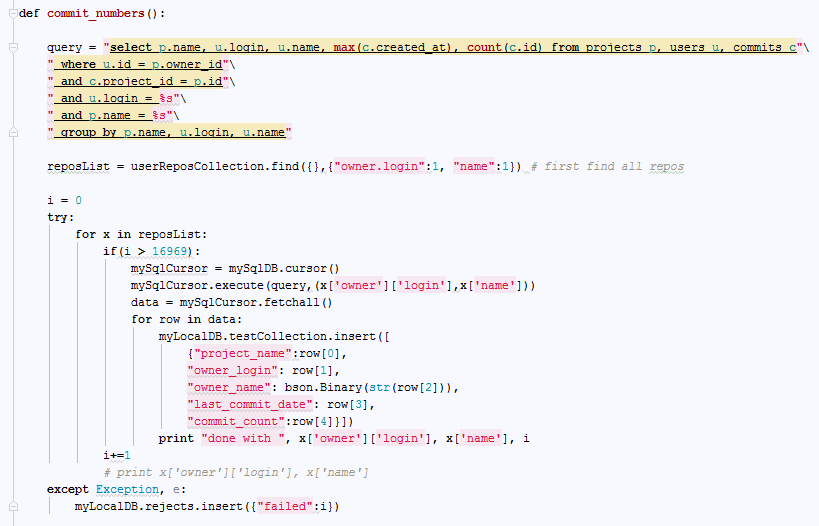
\includegraphics{Images/commitNumbers.PNG}
%}
%\caption{This Python script was used to collect the number of commits per local project.}
%\label{fig:commits-per-project}
%\end{center}
%\end{figure}

\subsection{Collecting Pull Requests}
\label{sec-pullreqs}
In order to determine overall user activity, we needed to understand how many pull requests had been submitted by each RTP user. For this, we pulled data directly out of the GHTorrent MySQL database and inserted it into our local MongoDB instance. The SQL query we used performed a union of two select statements. The first statement joins locally owned repositories on the head repository ID in the pull requests table and the second statement joins on the base repository id in the pull requests table. This is done to ensure we collect any repositories that have been forked. The script used for collecting the pull requests is shown in Figure \ref{fig:pullrequests}. 

\begin{figure}
\footnotesize
\begin{lstlisting}
def getPullReqs():

    query = "(select u.login, p.name, count(*) 
    	as 'prcount', 'head' as 'repotype'"\
            " from projects p, users u, pull_requests pr"\
            " where p.owner_id = u.id"\
            " and pr.head_repo_id = p.id"\
            " and p.deleted is false"\
            " and p.forked_from is null"\
            " and u.login = %s"\
            " group by p.id"\
            " order by count(*) desc)"\
            " UNION"\
            " (select u.login, p.name, count(*) 
            	as 'prcount', 'base' as 'repotype'"\
            " from projects p, users u, pull_requests pr"\
            " where p.owner_id = u.id"\
            " and pr.base_repo_id = p.id"\
            " and p.deleted is false"\
            " and p.forked_from is null"\
            " and u.login = %s"\
            " group by p.id"\
            " order by count(*) desc)"

    myUsers = githubRTPUsers.find({},{"login":1}) # first find all usernames

    i = 0
    try:
        for x in myUsers:
            mySqlCursor = mySqlDB.cursor()
            mySqlCursor.execute(query,(x['login'],x['login']))
            data = mySqlCursor.fetchall()
            for row in data:
                myLocalDB.calculated_pullReqByUser.insert([
                    {"login":row[0],
                    "name": row[1],
                    "prcount": row[2],
                    "repotype": row[3]}])
                print "done with ", x['login'], i
            i+=1
    except Exception, e:
        print e
        myLocalDB.rejects.insert({"failed":i})
\end{lstlisting}
\caption{Python script used to query for pull requests from the GHTorrent MySQL database and then insert them into our local MongoDB instance.}
\label{fig:pullrequests}
\end{figure}

\section{Social Networking - "Stargazing"}
\label{sec-stargazing}
In addition to overall open source activity, we were interested in understanding the popularity of local users and their work. One way to do this was to look into how many users had repositories which were being "starred" or "followed". We wrote a Python script to query the GHTorrent MongoDB instance (watchers collection), using our collected list of RTP users and their owned repositories. We inserted the results from this script into a new collection in our local MongoDB instance. Figure~\ref{fig:stargazers} shows an example of what one of these entries looks like. 

After the list of "stargazers" had been collected, we again used the MongoDB aggregation framework to find out which local repositories were the most popular.  Figure~\ref{fig:stargazers-count} shows what this query looked like. One thing to note for this collection is that if a user is a “contributor” on a project then the stars for that project end up in our list - some examples of this are shown in Chapter~\ref{Chapter:Findings} (Data Findings). Lastly, we utilized aggregation to find out how many followers each local user had (see Figure~\ref{fig:stargazing-aggregation}).

\begin{figure}
\tiny
\begin{lstlisting}
> db.githubRTPStargazers.findOne()
{
        "_id" : ObjectId("539eb518bd35432a2004564c"),
        "following_url" : "https://api.github.com/users/HagamosVideojuegos/following{/other_user}",
        "events_url" : "https://api.github.com/users/HagamosVideojuegos/events{/privacy}",
        "organizations_url" : "https://api.github.com/users/HagamosVideojuegos/orgs",
        "url" : "https://api.github.com/users/HagamosVideojuegos",
        "gists_url" : "https://api.github.com/users/HagamosVideojuegos/gists{/gist_id}",
        "html_url" : "https://github.com/HagamosVideojuegos",
        "subscriptions_url" : "https://api.github.com/users/HagamosVideojuegos/subscriptions",
        "repo" : "BombaFiesta-Unity3D-Futile",
        "owner" : "edbartley",
        "avatar_url" : "https://avatars.githubusercontent.com/u/6969130?",
        "repos_url" : "https://api.github.com/users/HagamosVideojuegos/repos",
        "received_events_url" : "https://api.github.com/users/HagamosVideojuegos/received_events",
        "gravatar_id" : "028308b2ed248bbd76fa686f0855006e",
        "starred_url" : "https://api.github.com/users/HagamosVideojuegos/starred{/owner}{/repo}",
        "site_admin" : false,
        "login" : "HagamosVideojuegos",
        "type" : "User",
        "id" : 6969130,
        "followers_url" : "https://api.github.com/users/HagamosVideojuegos/followers"
}
\end{lstlisting}
\caption{A view into the stargazers collection.}
\label{fig:stargazers}
\end{figure}

%\begin{figure}
%\begin{center}
%\resizebox{\textwidth}{!}{
%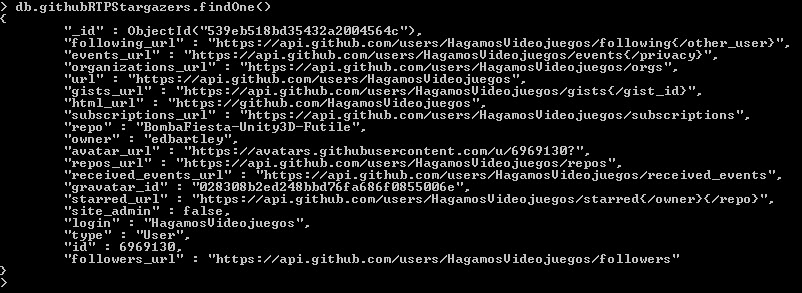
\includegraphics{Images/RTPStargazers_findOne.jpg}
%}
%\caption{A view into the stargazers collection.} 
%\label{fig:stargazers}
%\end{center}
%\end{figure}

\begin{figure}
\begin{lstlisting}
db.githubRTPStargazers.aggregate(
[
	{$group: {
    	_id:"$repo", 
        total: {$sum: 1}}},{$sort:{total:-1}
   	}
])
\end{lstlisting}
\caption{Aggregation used to find out how many followers each local repository contained.}
\label{fig:stargazers-count}
\end{figure}

\begin{figure}
\begin{lstlisting}
def stargazing():
    pip = [
        {"$group": {"_id": "$owner", "count": {"$sum": 1}}},
        {"$sort": SON([("count", -1), ("_id", -1)])},
        {"$project" : {"_id":1, "count":1, "owner":1,"repo":1}},
        {"$out" : "calculated_totalStargazers"}
    ]
    stargazersCollection.aggregate(pip)
\end{lstlisting}
\caption{Python script used to calculate the number of followers that each RTP user has.}
\label{fig:stargazing-aggregation}
\end{figure}

%\begin{figure}
%\begin{center}
%\resizebox{\textwidth}{!}{
%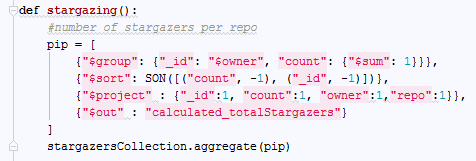
\includegraphics{Images/Stargazing-Aggregation.PNG}
%}
%\caption{Python script used to calculate the number of followers that each RTP user has.\label{fig:stargazing-aggregation}} 
%\end{center}
%\end{figure}

% !TEX root = main.tex
\chapter{Data Findings}
\label{Chapter:Findings}

Once the data collection method was developed and implemented, we started mining through the information collected in an attempt to answer the key questions described in chapter \ref{Chapter:Introduction} for the RTP region. We broke down those high level questions into more specific items described in section \ref{key-res-questions}. To find out about GitHub users in the RTP region, we provide answers to questions one through five. In order to see what the overall numbers look like in terms of projects developed out of the RTP area as well as their associated activity and current relevance, we answer questions six through twelve. Finally, in order to gain a better understanding of how RTP users are taking advantage of GitHub social networking features, as well as their overall popularity, we answer questions thirteen through fifteen.

We found that the easiest way to illustrate a lot of these findings was to create visual representations of the data collected. For this, we used Plot.ly, an open source framework for developing data visualizations in various languages \cite{_plotly_????}. Figure~\ref{fig:user-count-by-city-code} shows an example of the creation of a bar chart using this framework. The remainder of this chapter is broken down into specific sections dedicated to answering the key research questions. We first go into an overview of RTP users, then drill into RTP specific repositories, overall open source contribution activity and lastly look into the usage of social networking features available on GitHub.

\section{Key Research Questions}
\label{key-res-questions}
\begin{enumerate}
\item How many users does the RTP area have overall?
\item How many users does the RTP area have by type (User vs. Organization)?
\item What is the average number of repositories per user in RTP (overall)?
\item How long have local users been GitHub members? How many users have been around since GitHub started?
\item What city has the most users?
\item What is the repository count by User? 
\item What is the repository count by Organization?
\item Who has the most repositories overall in the RTP area?
\item Are users creating original repositories or forking existing repositories or collaborating more often?
\item What do the commit numbers look like for local RTP repositories?
\item How many of the RTP repositories are active (for this research, active is defined as repositories which contain changes that have been committed at some point over the last 6 months)?
\item What is the average life of a local project?
\item Are many local users being "followed"?
\item Are local repositories being starred often?
\item What are the most popular programming languages?
\end{enumerate}

\begin{figure}
\footnotesize
\begin{lstlisting}
def userCountByCity_BarChart():
    results = userCountByCity.find({"count":{"$gte" : 20}})

    x = []
    y = []

    for i in results:
        x.append(i['_id'])
        y.append(i['count'])

    plotly.offline.plot({
    "data": [
        Bar(x=x, y=y,
            marker=dict(
            color='rgb(158,202,225)',
            line=dict(
                color='rgb(8,48,107)',
                width=1.5
            ),
        ),
        opacity=0.6)
    ],
    "layout": Layout(
        title="Number Of Users By City (User Count Greater Than 20)",
        annotations=[
        dict(
            x=xi,
            y=yi,
            text=str(yi),
            xanchor='center',
            yanchor='bottom',
            showarrow=False,
        ) for xi, yi in zip(x, y)]
    )
    })
\end{lstlisting}
\normalsize
\caption{Sample Python code which pulls the total repository count per user using PyMongo and the Aggregation Framework.}
\label{fig:user-count-by-city-code}
\end{figure}

%\begin{figure}
%\begin{center}
%\resizebox{\textwidth}{!}{
%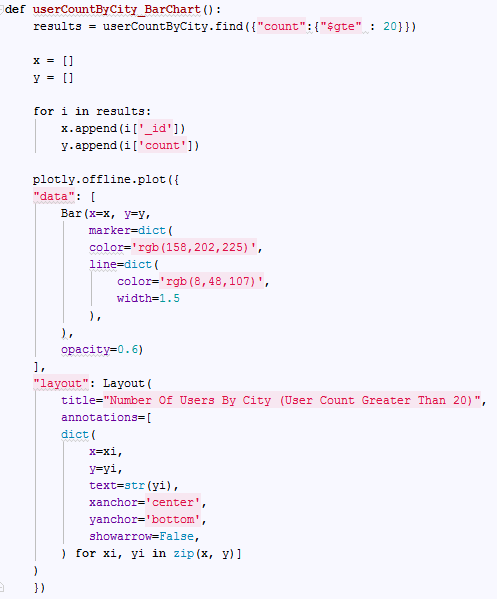
\includegraphics{Images/userCountByCity-pymongo.PNG}
%}
%\caption{Sample Python code which pulls the total repository count per user using PyMongo and the Aggregation Framework.} 
%\label{fig:user-count-by-city-code}
%\end{center}
%\end{figure}

%questions 1-5
\section{Users Overview}
In this section, we will focus on answering questions one through five from section \ref{key-res-questions}. We will find out how many users the RTP area has overall, by both User and Organization type. We will also find out how many repositories each user has on average, how long they have been members and which city in the region has the most users. The collection of RTP users was the most important dataset in this research as everything else was built upon them. As discussed in chapter \ref{Chapter:RTP}, RTP is a very prominent location for the information technology industry as a whole. We suspected we would find open source activity in the area but did not have any baselines from other locations to compare to. We managed to find 3,234 total RTP users (again, only being able to find users that had their location listed on GitHub). This means only .1\% of the RTP population (as also discussed in chapter 2, there are 3 million people living in a 60 mile radius of the park) are members of GitHub. Of these, 47 percent of them were located in Raleigh. Figure \ref{fig-userCountByCityBarChart} shows a bar chart created with Plot.ly with the number of RTP users by city. This chart only shows 8 cities as we filtered out all cities that had less than 20 users. Out of the 90 cities identified through NCLM (see \ref{fig:rtp-cities}), only 33 contained users contributing on GitHub. Raleigh, Durham and Chapel Hill had the highest number of users in the area which is understandable given these locations are home to the major research universities as well as many of the large technology companies referenced in chapter \ref{Chapter:RTP}. We also looked into the total number of RTP users by user type, finding that the majority of accounts were "User" - 2,982 with the remaining 252 being of type "Organization".

\begin{figure}
\begin{center}
\resizebox{\textwidth}{!}{
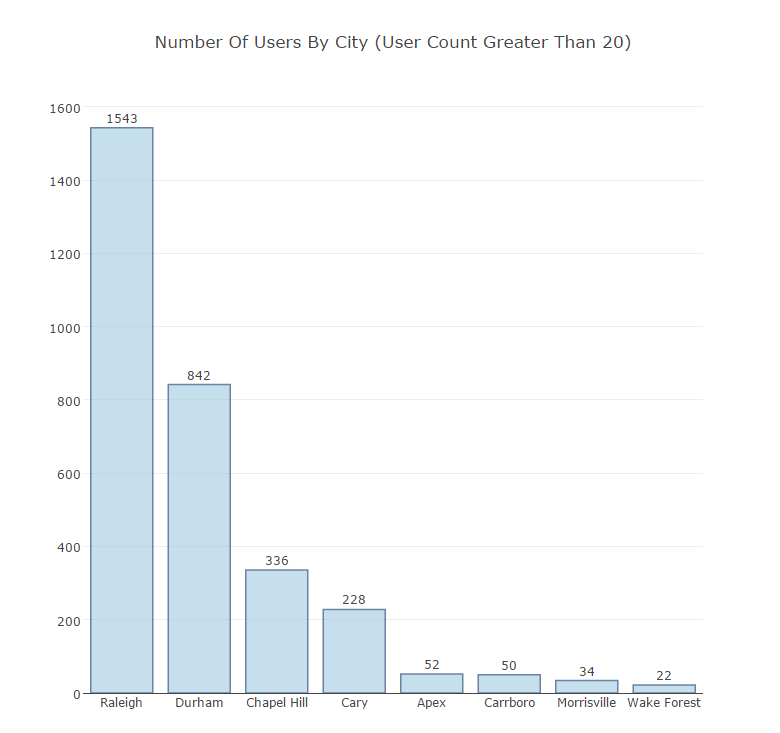
\includegraphics{Charts/userCountByCity-final.PNG}
}
\caption{This figure shows all RTP cities that have more than 20 users.} 
\label{fig-userCountByCityBarChart}
\end{center}
\end{figure}

Another metric that we were interested in gathering was how long the local RTP users had been members on GitHub. As mentioned in the previous chapter, GitHub has been around for 8 years now. We were curious to find out how many local users had created their accounts when the service went live. There ended up being around 130 users that have had their accounts for 7-8 years. Out of these accounts, 61\% (80 users) have been active (or submitted a commit) over the last 6 months. Figure \ref{fig-activeUsers} shows the script used to determine active users who have been members on GitHub for over 7 years. It was interesting to note that over half of the oldest users were still active on GitHub.

%\begin{figure}
%\label{fig-activeUsers}
%\begin{center}
%\resizebox{\textwidth}{!}{
%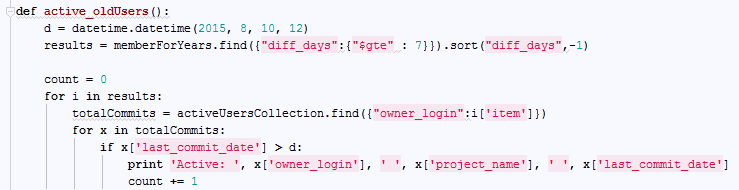
\includegraphics[width=16cm]{Images/active_legacyUsers.PNG}
%}
%\caption{This figure shows the Python script used to find RTP users that have been members on GitHub for more than 7 years and are still active today.} 
%\end{center}
%\end{figure}

\begin{figure}
\footnotesize
\begin{lstlisting}
def active_oldUsers():
  d = datetime.datetime(2015, 8, 10, 12)
  results = memberForYears.find({"diff_days":{"$gte" : 7}})
                          .sort("diff_days",-1)

  count = 0
  for i in results:
    totalCommits = activeUsersCollection.find({"owner_login":i['item']})
    for x in totalCommits:
        if x['last_commit_date'] > d:
            print 'Active: ', x['owner_login'], ' ', 
                              x['project_name'], ' ',
                              x['last_commit_date']
            count += 1
\end{lstlisting}
\caption{This figure shows the Python script used to find RTP users that have been members on GitHub for more than 7 years and are still active today.}
\label{fig-activeUsers}
\end{figure}

% questions 6-8
\section{Repositories Overview}
\label{sec:RepositoriesOverview}
In this section, we will present an overview of the RTP repositories found during the data collection phase through answering questions six through nine from section \ref{key-res-questions}. We will learn how many repositories have been created out of RTP (overall and by user type), as well as which RTP user has the most repositories. In total, we were able to find 34,825 total RTP user repositories. Of these, 31,843 were owned by a "User" type, while 2,982 were owned by an "Organization" type. There was a large amount of information available about each one of these repositories. Each repository contained an entry in a collection within our local MongoDB instance. These entries specified a number of items, including the owner details, the number of forks, whether or not the repository was a fork itself, the programming language used, the number of watchers, the create date, last updated date, as well as several API URLs that could be used to perform a number of actions on GitHub (view comment, view issues, view events, download the repository, etc.).

We calculated that RTP users have created an average of 12 repositories. The user with the most repositories had created 351, while there were a large number of users that had only created one repository. Figure \ref{fig-repoCountByUser-highest} is a chart created to show the users with the most repositories (breaking it down to users with more than 120 owned repositories). This does not necessarily mean they are active repositories and in fact could have been created and only used as a means of storage and never opened up for collaboration nor as a source code repository. The user with the most number of repositories was created as an "Organization", the account is still active today but not all 351 repositories are currently being contributed to. We will assess the activity of all repositories in section \ref{sec-ActivityOverview}. 

\begin{figure}
\resizebox{\textwidth}{!}{
\begin{bchart}[max=351]
\bcbar[text=pixbit,
 color=blue!20]{351}
\bcbar[text=jmxpearson, color=blue!20]{223}
\bcbar[text=battlemidget, color=blue!20]{193}
\bcbar[text=BanzaiMan, color=blue!20]{192}
\bcbar[text=apsaltis, color=blue!20]{155}
\bcbar[text=Rleahy22, color=blue!20]{151}
\bcbar[text=connyay, color=blue!20]{139}
\bcbar[text=vbatts, color=blue!20]{131}
\bcbar[text=pmuellr, color=blue!20]{131}
\bcbar[text=thewtex, color=blue!20]{129}
\bcbar[text=jcfr, color=blue!20]{127}
\bcbar[text=ryanfb, color=blue!20]{121}
\bcxlabel{Repository Count By User}
 \end{bchart}
}
\caption{This bar chart shows users with the most overall repositories in the RTP region.}
\label{fig-repoCountByUser-highest}
\end{figure}
             
The next piece of information gathered about overall repositories in the RTP region was the total number of original versus forked projects. We were interested in understanding if users created original projects more often than forking from already existing projects. Table \ref{fig-forked-repos} and \ref{fig-orig-repos} show the findings from these calculations. After sampling this data, we found out that around 40\% of the projects in RTP are forked and 59\% are original. This does not exclude inactive repositories. What this tells us is that while more than half of the repositories are original projects created by the RTP owner, there are still a large number of projects that have been forked from already existing projects with a possible intent to collaborate.

\begin{table}
\parbox{.45\linewidth}{
\centering
\begin{tabular}{|c|c|}
\hline
Forked Repositories & Total Users\\
\hline
15,244 & 2099\\
\hline
\end{tabular}
\caption{Total Original Repositories in RTP}
\label{fig-forked-repos}
}
\hfill
\parbox{.45\linewidth}{
\centering
\begin{tabular}{|c|c|}
\hline
Original Repositories & Total Users\\
\hline
19,745 & 2518\\
\hline
\end{tabular}
\caption{Total Forked Repositories in RTP}
\label{fig-orig-repos}
}
\end{table}

% 10-11
\section{Activity Overview}
\label{sec-ActivityOverview}
We did some investigating into how many local users were active while seeking to answer questions ten and eleven. We find out what the commit numbers look like for RTP repositories, as well as the overall activity of RTP users. As discussed previously, we defined a user as being "active" if they  have made a commit sometime over the last 6 months. We found that 2,559 unique users had made a commit over the last 6 months on GitHub which we seemed quite high. We can't necessarily say that 79\% of RTP users are active on GitHub, however, due to the fact that was discussed in chapter \ref{Chapter:Background}, when committing a change in GitHub, the author field is free text in many cases. We can see this quite clearly in the collected dataset on commits. There are unfortunately many users who lazily entered data such as their first name only (i.e. "Ben") instead of their full name, e-mail address or login name as an identifier. As part of future research, it would be useful to programatically attempt to match authors to their rightful GitHub account, similar to what the GHTorrent project does (as discussed already in section \ref{sec-GHTorrentProject}). This way we would be able to calculate a more accurate number on the total number of active users in the area.

We were able to say for certain that there are 6,756 unique RTP owned repositories that are active on GitHub, since this field cannot be free text. This means that of all the repositories owned by RTP users, 19\% of them are active. Figure \ref{fig-projCommits6mon} shows all users with more than 2,000 commits over the last 6 months. We looked a bit further into the top 10 active users (by login ID) to find out more information about them. All 10 of these users have made more than 2,000 commits to projects over the last 6 months (see Table \ref{table-top10activeusers}). As we can see, 70\% of these users are set up as Organizations on GitHub, which makes sense in that there would be more commits than "User" projects where there may be only one contributor. It was hard to identify a specific trend between these numbers. For example, these project owners either heavily utilize pull requests, or they don't. This observation could be explained by the fact that users and organizations utilize different workflows as already discussed in section \ref{sec-GitHub}.


\begin{figure}
%\resizebox{\textwidth}{!}{
\begin{bchart}[max=11.312,width=.9\textwidth]
\bcbar[text=OpenNMS, color=blue!20, value=11312]{11.312}
\bcbar[text=tee3, color=blue!20, value=3665]{3.665}
\bcbar[text=bredelings, color=blue!20, value=3145]{3.145}
\bcbar[text=duke-libraries, color=blue!20, value=2809]{2.809}
\bcbar[text=mautic, color=blue!20, value=2788]{2.788}
\bcbar[text=caktus, color=blue!20, value=2738]{2.738}
\bcbar[text=automatak, color=blue!20, value=2684]{2.684}
\bcbar[text=waldenraines, color=blue!20, value=2407]{2.407}
\bcbar[text=pencilblue, color=blue!20, value=2357]{2.357}
\bcbar[text=UNC-Libraries, color=blue!20, value=2234]{2.234}
\bcbar[text=jhinkey, color=blue!20, value=2149]{2.149}
\bcbar[text=deads2k, color=blue!20, value=2077]{2.077}
\bcxlabel{Total Commits per User}
 \end{bchart}
%}
\caption{This figure shows all users with more than 1000 commits over the last 6 months.}
\label{fig-projCommits6mon}
\end{figure}


\begin{table}
\centering
\resizebox{\textwidth}{!}{
\begin{tabular}{|c|c|c|c|c|c|c|}
\hline
User ID & User Type & Member Since & City & \# Projects & \# Pull Reqs & \# Stargazers \\
\hline
OpenNMS & Organization & Dec-12 & Pittsboro & 66 & 864 & 254 \\
\hline
tee3 & User & Mar-10 & Raleigh & 18 & 2 & 5 \\
\hline
bredelings & User & Oct-09 & Durham & 8 & 2 & 15 \\
\hline
duke-libraries & Organization & Oct-12 & Durham & 52 & 2310 & 40 \\
\hline
mautic & Organization & Aug-13 & Raleigh & 14 & 718 & 479 \\
\hline
caktus & Organization & Apr-10 & Durham & 89 & 1602 & 856 \\
\hline
automatak & Organization & Jan-13 & Raleigh & 10 & 42 & 81\\
\hline
waldenraines & User & Apr-13 & Raleigh & 17 & 0 & 0 \\ 
\hline
pencilblue & Organization & Feb-14 & Raleigh & 15 & 751 & 1257 \\
\hline
UNC-Libraries & Organization & Jan-11 & Chapel Hill & 28 & 766 & 157 \\
\hline
\end{tabular}
}
\caption{More information on the top 10 active RTP users (have pushed commits in the last 6 months). This chart shows their total number of projects, pull requests and stargazers. }
\label{table-top10activeusers}
\end{table} 

%12-14
\section{Popularity Overview}
\label{sec-PopularityOverview}
Finally, after reviewing metrics on RTP users, their repositories and overall activity on GitHub, we decided to take a look into the data to find out how "popular" our local users and projects were. In this section, we will discuss questions twelve through fifteen. We will seek to find out if many RTP users are being "followed" or "starred". We will also find out what the most popular programming language is. As mentioned in chapter \ref{Chapter:Background}, GitHub gives us an easy way to do this with their built in social media features such as "stargazing". We were able to dig into the collected data to find out that some of our users are actually somewhat popular. 1,253 users (39\%) contain at least one follower. We have 2 local users that have more than 10,000 followers. Figure \ref{fig-stargazersByUser} gives us a view of the number of stargazers that each user has (where the total number of followers is greater than 1000). The RTP user with the most stargazers is an author of a book on PHP, who lives and works in Chapel Hill.

\begin{figure}
%\resizebox{\textwidth}{!}{
\begin{bchart}[max=125.71,width=.9\textwidth]
\bcbar[text=codeguy, color=blue!20, value=12571]{125.71}
\bcbar[text=fogleman, color=blue!20, value=11682]{120.82}
\bcbar[text=jlong, color=blue!20, value=7856]{80.56}
\bcbar[text=alebcay, color=blue!20, value=6249]{70.49}
\bcbar[text=twotoasters, color=blue!20, value=3798]{60.98}
\bcbar[text=cognitect, color=blue!20, value=2586]{55.86}
\bcbar[text=smashingboxes, color=blue!20, value=2428]{50.28}
\bcbar[text=jaymedavis, color=blue!20, value=1564]{45.64}
\bcbar[text=clojure-cookbook, color=blue!20, value=1554]{40.54}
\bcbar[text=alandipert, color=blue!20, value=1553]{39.53}
\bcbar[text=mapier, color=blue!20, value=1304]{35.04}
\bcbar[text=pencilblue, color=blue!20, value=1257]{33.57}
\bcbar[text=kconner, color=blue!20, value=1204]{31.04}
\bcbar[text=stuarthalloway, color=blue!20, value=1187]{29.87}
\bcbar[text=bwsewell, color=blue!20, value=1145]{27.45}
\bcbar[text=yfactorial, color=blue!20, value=1073]{24.073}
\bcxlabel{Total Stargazers per User}
 \end{bchart}
%}
\caption{This figure shows the number of followers that each user has (where the count of followers is greater than 1000).}
\label{fig-stargazersByUser}
\end{figure}

Another metric we collected was the overall programming language popularity in this region. We aggregated the repository collections and counted the number of occurrences for each language, ignoring any projects that did not have the programming language listed (8,459 or 24\% did not have one listed). Figure \ref{fig-progLangPopularity} shows the number of projects that use each language in a bar chart where usage count is greater than 1,000, with JavaScript leading the way. We note that this information is what comes back from GitHub, it is important to remember that many projects will likely have more than one associated programming language.

\begin{figure}
%\resizebox{\textwidth}{!}{
\begin{bchart}[max=5.467,width=.9\textwidth]
\bcbar[text=JavaScript, color=blue!20, value=5467]{5.467}
\bcbar[text=Ruby, color=blue!20, value=4527]{4.527}
\bcbar[text=Python, color=blue!20, value=3457]{3.457}
\bcbar[text=Java, color=blue!20, value=2062]{2.062}
\bcbar[text=CSS, color=blue!20, value=1349]{1.349}
\bcbar[text=PHP, color=blue!20, value=1255]{1.255}
\bcbar[text=Shell, color=blue!20, value=1069]{1.069}
\bcxlabel{Top GitHub Programming Languages in RTP}
 \end{bchart}
%}
\caption{This figure shows the most popular programming languages in the RTP region, where the usage count is greater than 1000.}
\label{fig-progLangPopularity}
\end{figure}


%15
\section{Average Life of a RTP Project}
\label{sec-lifeOfAProj}
One of the additional data points that we decided to collect was what the average life of a GitHub project owned by a user in RTP looked like (question fifteen). We found out that the oldest RTP repository was created less than a month after GitHub was founded, "depth-charge". Figure \ref{fig-mongoqueryOldestRTPRepo} shows the query used to find this information in our local MongoDB database. This particular repository was created 8 years ago and hasn't been updated since.

\begin{figure}
\label{fig-mongoqueryOldestRTPRepo}
\begin{lstlisting}
> db.githubRTPUsersRepos
	.find({},
    	{"owner.login":1,"created_at":"1","name":1})
    .sort({"created_at":1})
    .limit(1)
> { 
	"_id" : ObjectId("52bedd67bd3543677400823a"), 
	"owner" : { "login" : "bscofield" }, 
    	"name" : "depth-charge", 
    	"created_at" : ISODate("2008-02-27T12:42:10Z") 
  }
\end{lstlisting}
\caption{Finding the oldest RTP repository from MongoDB's shell  (query and result).}
\end{figure}

Finally, we also found that the average life of a RTP project is 102 days. This was calculated by subtracting the created date from the last commit date and then averaging the entire gathered list. We found that the shortest project was 1 day and that there are plenty of projects that are still ongoing and active.

\section{Threats to Validity}
Due to the quality of data that we were able to retrieve for this project, there are several threats to validity that must be mentioned. As already discussed, it is important to remember that the location field in GitHub is not required, hence there is likely a large population of users that are left out of our research because they haven't given a location or have possibly given an inaccurate one. This was a limitation with our research due to the fact that we were heavily interested in querying for users that lived in such a specific location. Additionally, it was difficult for us to find out the exact number of commits per user. This is because users are able to enter free text into the authors field when committing a change in the GitHub shell (command line). This impacted the results from the mining for overall activity in the RTP region. We looked into pulling data from other sources to supplement the information from GitHub. An example source being LinkedIn, which was unsuccessful due to restrictions with the licensing of their REST API.

% !TEX root = main.tex
\chapter{Conclusion}
\label{Chapter:Conclusion}

The purpose of this research was to shed light on the open source activities in the Research Triangle Park region using information mined from  GitHub. We began the data collection phase by gathering metrics around how many people in the RTP area were involved in open source projects (from both personal and organizational levels). This information was then used to explore repositories developed out of the RTP area, looking into characteristics such as the programming languages used, their associated activity, and current relevance of the various projects. Lastly, we explored how RTP users were involved in the social media aspects of GitHub. In summary, we found that, as a whole, the RTP region is not heavily involved in the open source community, but we were able to identify a number of users that were prominent on the platform both from the single user and organizational perspective.

As part of future research, it would be interesting to extend these experiments to cover other locations with a similar technology industry profile, providing additional context for the current results and providing insight into how open source development differs in different parts of the United States and in technology hubs in other countries. It would also be interesting to add a temporal aspect to this research, exploring how open source development activities change over time. Teams and individual developers could also use this work to find out which cities have the most users, repositories, open source activity, and overall popularity, potentially by providing this data through a portal. Lastly, it would also be interesting to compare findings such as the most popular programming languages to the job requirements in the local markets to see if any trends can be identified. The scripts developed for this thesis, used as part of the data collection and analysis phases, are themselves available on GitHub under an open-source license.



\bibliographystyle{IEEEtran}
\bibliography{cited}

\coversheet

\end{document}


% MH: PRIOR CONTENTS HERE
% \documentclass[11pt,          % font size: 11pt or 12pt
%                ms,           % degree:    ms or phd
%                doublespacing % spacing: onehalfspacing or doublespacing
%                ]{ncsuthesis}

% %%----------------------------------------------------------------------------%%
% %%------------------------------ Import Packages -----------------------------%%
% %%----------------------------------------------------------------------------%%
% \usepackage{afterpage}
% \usepackage{ragged2e}
% \usepackage{booktabs}  % professionally typeset tables
% \usepackage{amsmath}%,amssymb,amsfonts}
% \usepackage{textcomp}  % better copyright sign, among other things
% %\usepackage{xcolor}
% \usepackage{lipsum}    % filler text
% \usepackage{subfig}    % composite figures
% \usepackage{listings}
% \usepackage{float}
% \usepackage{algorithm}
% %\usepackage{algorithmic}
% \usepackage{algpseudocode}
% \usepackage{soul}
% \usepackage{indentfirst}
% \usepackage{multicol}


% %\usepackage{ulem}
% %%%%%%%%%%% Hack for alphanumeric bibliography
% \RequirePackage[
% 			style=alphabetic,%numeric-comp,%authoryear-comp,%
% 			sorting=nyt,%ynt					
% 			hyperref=true, %	
% 			firstinits=true,%
% 			backend=bibtex,
% 			natbib=true,
% 			url=false,
% 			isbn=false,
% 			maxnames=2, %for et al to be used
% 			maxalphanames=1, %to avoid printing a + for every et al in the abbreviation
% 			doi=false]{biblatex}		
	
% \newcommand{\beginCode}[3]{\begin{lstlisting}[caption={{#1}},captionpos=bottom,label={#2},frame=lines,numbers=right]{#3}}
% \newcommand{\stopCode}{\end{lstlisting}}		

% %Added by Lindsey (issues with asterisk in code otherwise)
% \renewcommand{\textasteriskcentered}{\ensuremath{*}}

% \addbibresource{Zotero.bib}

%  \defbibheading{myheading}[BIBLIOGRAPHY]{
%  \chapter*{#1}
%  %\centerline{\bf{#1}}
%  \markboth{#1}{#1}}

% %\usepackage{amsmath,amssymb,amsfonts} %amssymb and amsfonts cannot be used in conjunction with mdput
% %\usepackage{graphicx,subfig}% Include figure files
% \usepackage{dcolumn}% Align table columns on decimal point
% \usepackage{bm}% bold math
% %\usepackage{hyperref}% add hypertext capabilities
% %\usepackage{hypernat}% make hyperref and natbib work together
% \usepackage{cancel}
% \usepackage{verbatim}% multiline commenting
% \usepackage{ifthen}
% \usepackage{url}
% \usepackage{sectsty}
% \usepackage{balance} 
% %\usepackage{caption}
% \usepackage{graphicx} %eps figures can be used instead
% \usepackage{lastpage}
% \usepackage[format=plain,justification=RaggedRight,singlelinecheck=false,font=small,labelfont=bf,labelsep=space]{caption} 
% \usepackage{fancyhdr}
% \pagestyle{fancy}

% %http://tex.stackexchange.com/questions/100817/error-when-using-bc-from-abbrevs-in-caption
% %Getting BC
% \usepackage{abbrevs}
% \usepackage{etoolbox}

% \usepackage{units} %Needed to solve bug from citation Hydrodynamics in 21/2 dimensions
% %see http://www.latex-community.org/viewtopic.php?f=5&t=989

% \usepackage[sharp]{easylist} %used for brainstorming purposes 
% %============================================================================
% % Adding packages from else-where to here..

% \usepackage[parfill]{parskip}              

% \usepackage[table]{xcolor}
% \usepackage{array,booktabs}
% \usepackage{colortbl}
% \usepackage{pdflscape}
% \usepackage{tikz}
% \usepackage{placeins}
% \usepackage{titlesec}
% \usepackage{color}
% \usepackage{calc}
% %============================================================================
% % for emptying pages on list of figures and tables
% \makeatletter
% \newcommand{\emptypage}[1]{%
%   \cleardoublepage
%   \begingroup
%   \let\ps@plain\ps@empty
%   \pagestyle{empty}
%   #1
%   \cleardoublepage}
% \makeatletter
% %============================================================================


% \robustify{\DateMark} % after having loaded abbrevs

% \newcolumntype{L}{@{}>{\kern\tabcolsep}l<{\kern\tabcolsep}}


% \setcounter{secnumdepth}{4}

% \titleformat{\paragraph}
% {\normalfont\normalsize\bfseries}{\theparagraph}{1em}{}
% \titlespacing*{\paragraph}
% {0pt}{3.25ex plus 1ex minus .2ex}{1.5ex plus .2ex}

% \dispositionformat{\bfseries}            % bold and serif

% \headingformat{\large\MakeUppercase}   % All letters uppercase
% \frenchspacing


% %%  Optional Packages to consider.   These packages are compatible with
%%    ncsuthesis.  

%% -------------------------------------------------------------------------- %%
%% Fancy chapter headings
%%  available options: Sonny, Lenny, Glenn, Conny, Rejne, Bjarne
\usepackage[Sonny]{fncychap}

%%----------------------------------------------------------------------------%%
%% Hyperref package creates PDF metadata and hyperlinks in Table of Contents
%%  and citations.  Based on feedback from the NCSU thesis editor, 
%%  the links are not visually distinct from normal text (i.e. no change
%%  in color or extra boxes).
\usepackage[
  pdfauthor={John Mark Smith},
  pdftitle={The Title},
  pdfcreator={pdftex},
  pdfsubject={NC State ETD Thesis},
  pdfkeywords={keyword1, keyword2},
  colorlinks=true,
  linkcolor=black,
  citecolor=black,
  filecolor=black,
  urlcolor=black,
]{hyperref}


%% -------------------------------------------------------------------------- %%
%% Microtype - If you use pdfTeX to compile your thesis, you can use
%%              the microtype package to access advanced typographic
%%              features.  By default, using the microtype package enables
%%              character protrusion (placing glyphs a hair past the right 
%%              margin to make a visually straighter edge)
%%              and font expansion (adjusting font width slightly to get 
%%              more favorable justification).
%%              Using microtype should decrease the number of lines
%%              ending in hyphens.
\usepackage{microtype}


%%----------------------------------------------------------------------------%%
%% Fonts 

%% ETD guidelines don't specify the font.  You can enable the fonts
%%  by uncommenting the appropriate lines.  Using the default Computer 
%%  Modern fonts is *not* required.  A few common choices are below.
%%  See http://www.tug.dk/FontCatalogue/ for more options.

%% Serif Fonts -------------------------------------------------
%%  The four serif fonts listed here (Utopia, Palatino, Kerkis,
%%  and Times) all have math support.


%% Utopia
\usepackage[T1]{fontenc}
\usepackage[adobe-utopia]{mathdesign}

%% Palatino
%\usepackage[T1]{fontenc}
%\usepackage[sc]{mathpazo}
%\linespread{1.05}

%% Kerkis
%\usepackage[T1]{fontenc}
%\usepackage{kmath,kerkis}

%% Times
%\usepackage[T1]{fontenc}
%\usepackage{mathptmx}


%% Sans serif fonts -------------------------

%\usepackage[scaled]{helvet}  % Helvetica
%\usepackage[scaled]{berasans} % Bera Sans

% \setlength{\headheight}{14pt}

% %%---------------------------- Content Options -------------------------------%%
% \committeesize{3}

% \chair{Mark Hills, PhD.}
% \memberI{Nasseh Tabrizi, PhD.}
% \memberII{Junhua Ding, PhD.}

% \student{Lindsey}{Lanier} % a full middle name
% \program{Software Engineering}

% %% Thesis Title
% \thesistitle{Software Engineering as a Social Process: \\A Study of Research Triangle Park}

% %% Capital letter height
% % \newlength{\chaptercapitalheight}
% % \settoheight{\chaptercapitalheight}{D}
% % \newlength{\chapterfootskip}
% % \setlength{\chapterfootskip}{\chaptercapitalheight}
% % \addtolength{\chapterfootskip}{2\baselineskip}
% % \addtolength{\chapterfootskip}{0.5ex}  % A little extra space to ensure there are 2 full double spaced lines
% % \renewcommand{\listfigurename}{LIST OF FIGURES}
% % \renewcommand{\listtablename}{LIST OF TABLES}
% % \renewcommand{\bibname}{BIBLIOGRAPHY}

% % \newlength\graphht
% % \newcommand\calculategraphicstargetheight[1]{%
% %      \setlength\graphht{\textheight 
% %                        -\parskip
% %                        -\abovecaptionskip -\belowcaptionskip
% %                        -(12pt * #1) % assuming baselineskip of 12pt in caption
% %                        -\chapterfootskip
% %                        }}
% % \fancypagestyle{lscapedplain}{%
% %   \fancyhf{}
% %   \fancyfoot{%
% %     \tikz[remember picture,overlay]
% %       \node[outer sep=1cm,above,rotate=90] at (current page.east) {\thepage};}
% % \renewcommand{\headrulewidth}{0pt} 
% % \renewcommand{\footrulewidth}{0pt}
% % }

% % \setlength\parindent{0pt}
   
% \begin{document}
% \pagestyle{plain}
% \lstset{language=Java}
% %%---------------------------------------------------------------------------%%
% \frontmatter

% %% ------------------------------ Abstract ---------------------------------- %%
\begin{abstract}

Research Triangle Park, NC is one of the largest research parks in the world, and the largest in the United States. Within the 7,000 acre park, there are currently more than 200 companies employing around 50,000 people in a number of fields of expertise---information technology playing a large role. This research is aimed at utilizing public data from GitHub and other sources to gain a better understanding of what the software engineering, particularly open source, demographic looks like in such a prominent location. \# of 


\end{abstract}


%% ---------------------------- Copyright page ------------------------------ %%
%% Comment the next line if you don't want the copyright page included.
%\makecopyrightpage

%% -------------------------------- Title page ------------------------------ %%
\maketitlepage

%% -------------------------------- Dedication ------------------------------ %%
\begin{dedication}
 \centering To my parents.
\end{dedication}

%% -------------------------------- Biography ------------------------------- %%
\begin{biography}
The author was born in a small town \ldots
\end{biography}

%% ----------------------------- Acknowledgements --------------------------- %%
\begin{acknowledgements}
I would like to thank my advisor for his help.
\end{acknowledgements}


\thesistableofcontents

\thesislistoftables

\thesislistoffigures


% %%---------------------------------------------------------------------------%%
% \mainmatter

% % \floatstyle{boxed}
% % \restylefloat{figure}
% % \addtocontents{toc}{\protect\thispagestyle{empty}}

% % \pagestyle{fancy}
% % \newgeometry{margin=1in,lmargin=1.25in,footskip=\chapterfootskip, includehead, includefoot}
% % !TEX root = main.tex
\chapter{Introduction}
\label{Chapter:Introduction}

Open source software development is continuing to grow within information technology communities. The data capable of being extracted from collaborative development platforms gives researchers an opportunity to answer many questions about open source project activity and trends. However, at this point in time, we know little about how people are participating in open source development from a regional perspective. This research is aimed at studying open source activities through public data within GitHub \cite{_github_2016} to understand what the open source software engineering demographic looks like in Research Triangle Park (RTP), NC, one of the most prominent research parks in the world. 

GitHub is a widely used platform for open source software development and collaboration. Its extensive features give software developers the capability to join forces with others from all over the world on a variety of projects, from small projects to major projects that are being used at the enterprise level. GitHub provides a public REST API which grants researchers the opportunity to mine and study this data from an empirical perspective. Using the GHTorrent Project \cite{gousios_ghtorrent:_2012}, \cite{gousios_ghtorent_2013} as our foundation for information, we focus on answering a few key questions throughout this research:
\begin{enumerate}
\item What do the metrics look like around individual users and organizations and their involvement in open source projects in the RTP area? 
\item What do the overall numbers look like with regards to projects being developed by users and organizations in the RTP region? How active are these projects, and are they still relevant since inception?  
\item How do users and organizations in the RTP region use the social media features available on GitHub?
\end{enumerate}

While the answers to these questions have focused on the RTP region, the scripts developed for this empirical study can also, with some generalization, be used to study other geographic areas, which will enable future research including answering similar questions for other regions and comparing multiple regions. Chapter 2 will go through key reasons on why RTP was chosen as a strategic location for this research. Chapter 3 will provide more information around GitHub, with an overview of terms and associated workflows, as well as an overview of the GHTorrent project. Chapter 4 will discuss related research on this topic, particularly studies into open source data. Chapter 5 and 6 will go through the methodologies used for data collection and then provide analysis of the RTP data collected. Lastly, we will wrap up in Chapter 7 with closing remarks about this research and ideas for future research. 

\paragraph{Research Contribution:} Through empirical techniques applied to data mined from project repositories on GitHub, this thesis quantitatively shows how both individual developers and organizations participate in open source software development in the Research Triangle Park region of North Carolina. The process used to extract and compute over the repository data has been scripted to ensure the reported results can be easily replicated, while the scripts themselves have been designed to enable future studies of other technology regions as well as comparative studies of multiple regions. The data collection tools and techniques created to enable this research are publicly available on GitHub (User ID: LindseyKLanier, \cite{_lindsey_github}) under an open-source license. 
% % !TEX root = main.tex
\chapter{Overview of Research Triangle Park}
\label{Chapter:RTP}

In this chapter, we first define Research Triangle Park, the region studied in this thesis. We then explain why this region was chosen for this study, focusing on the rapid growth of the region and the significant presence of high tech companies and major universities.

\section{Where is Research Triangle Park?}
Research Triangle Park (RTP) is the largest research and science park in North America, and one of the largest in the world. The park, which stretches 7,000 acres across Wake and Durham counties was founded in 1959 by the Research Triangle Foundation. RTP is not a city, but it has its own special county district \cite{_research_????}. The Research Triangle Region Organization, a partnership dedicated to overseeing collaboration between businesses, government and various other institutions within the region identifies RTP as the following counties (see Figure \ref{fig:rtp-region}): Chatham, Durham, Edgecombe, Franklin, Granville, Harnett, Johnston, Lee, Moore, Nash, Orange, Person, Vance, Wake, Warren, and Wilson \cite{_research_????}. Additionally, the RTP Organization has stated that the RTP metro area has a population of 1.3 million people, and that there are 3 million people within a 60-mile radius of the park \cite{weddle_research_????}. Our project utilized public NC League of Municipalities (NCLM) data to identify all of the cities in each of the RTP counties to assist our research \cite{_north_????}.

\begin{figure}
\begin{center}
\resizebox{\textwidth}{!}{
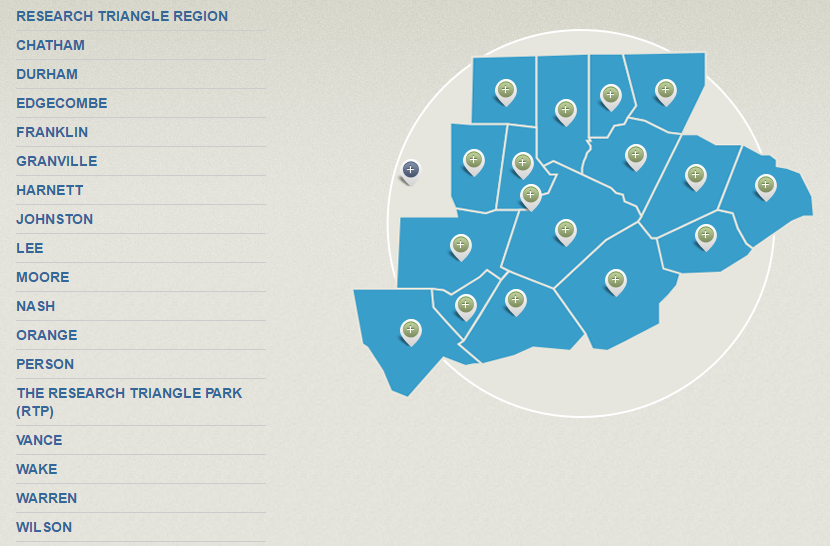
\includegraphics{Images/RTP-Region_2.png}
}
\caption{RTP region as defined by Research Triangle Region Organization \cite{_research_????}}
\label{fig:rtp-region}
\end{center}
\end{figure}

\section{Why Research Triangle Park?}

Many reasons can be attributed to our choosing of RTP and its surrounding communities for initial research into local open source activities. Over the last decade, numerous media outlets and journalists have continuously given this region nicknames such as “Start-up Capital of the South” \cite{_durhams_????} and “The Next Silicon Valley” \cite{_4_????}. Between 2000 and 2012, Raleigh's population grew 47.8 percent, which topped Forbes's list of fastest growing metropolitan areas in the country. This number was more than three times the overall growth of all other metropolitan areas \cite{kotkin_americas_????}. The Google for Entrepreneurs Network has invested in 3 different locations in Raleigh/Durham (RDU) for what they call "American Underground". American Underground is referred to as a "Start-Up Incubator" where software groups can rent space for their teams to meet and work \cite{_american_????}. The Research Triangle Park Organization continues to drive their mission to "change the course of history" by bringing people together and fostering innovation and creativity in the RTP community \cite{_research_2016}. They've recently open up a new center, The Frontier, with free space for teams to collaborate and participate in a variety of networking events \cite{_frontier_????}. 

Outside of the start-up communities, many big technology players have a presence in RTP--Red Hat, Citrix, Cisco, NetApp, IBM, Microsoft, Google, SAS, and others,  with more news about others following every year. There are several local prestigious universities including the University of North Carolina Chapel Hill, North Carolina State University, and Duke University, all of which are consistently producing top talent within the science, math and technology industries. According to the Research Triangle Park Organization \cite{_research_2016}, local companies and organizations have won Nobel Prizes and the Pulitzer. To date, they've recorded that there have been 245 company start-ups, 3,256 patents, and 1,970 trademarks. 

At the beginning of 2016, the North Carolina State of Technology Industry Report was released. We found some of the statistics produced by this group (NC Technology Association and Economic Leadership of Raleigh) relevant to reasons we chose the RTP region, even though they were specific to the state as a whole \cite{_nc_????}. 

A few of the highlights from this report included:

\begin{itemize}  
\item North Carolina is the \#2 state in Information Technology (IT) employment growth from 2009-2014.
\item North Carolina is the \#4 state for University Technology Licenses and Options Executed with 242 licenses and options in 2014.
\item Future North Carolina tech sector growth is expected to outpace national and American South averages.
\item Over the past year technology employment grew by 3.6 percent, and technology establishments grew by 5.2 percent.
\end{itemize}

These statistics can serve as a proxy for choosing to do research on other areas with a large and growing presence in the information technology industry.

% % !TEX root = main.tex
\chapter{GitHub and The GHTorrent Project}
\label{Chapter:Background}

In this chapter, we will give an overview of GitHub as a platform as well as the GHTorrent project and it's associated data source. GitHub and GHTorrent provide data which is the foundation to the research performed in this thesis.

\section{GitHub}
\label{sec-GitHub}
GitHub is a web-based platform used for version control and collaboration between developers. Users can choose to utilize standard Git commands in a terminal to manage their code on GitHub or use the GitHub graphical user interface (GUI) and associated features on GitHub.com. As of February 2016, there were 12 million people collaborating across 31 million repositories on GitHub \cite{_github_2016}. Users wanting to create a GitHub account for their projects have two options, public (free) and private (paid). Public repositories are heavily used by open-source teams to allow for code storage and collaboration from users all over the world. GitHub gives users the option to create "organizations" to more easily manage teams. Organizations allow teams to group one or more projects under one umbrella. Multiple owners can be mapped to organizations for settings and permissions management. 

This research pulls data on GitHub's source code management features with a focus on mining RTP specific statistics as well as looking into the involvement that RTP users have in the social networking aspect of the platform. Source code packages hosted on GitHub are referred to as repositories. We utilize the GHTorrent Project \cite{gousios_ghtorent_2013} for data collection of RTP specific (public) repositories. Public repositories can be browsed and contributed to by not only the owner but anyone else interested in downloading a local copy. Changes by GitHub users can be submitted to the repository owner for review in the form of a "pull request". Changes are saved to repositories through what are known as "commits". There are various workflows that could be implemented for GitHub projects. One popular option is to utilize "forking" and "pull requests". A "fork" is a clone of a repository, saved as a new repository on one's own GitHub account. Users might implement their own enhancement to the cloned application, or could also work on an associated "issue". One or more commits can be pushed to this clone. Once the developer is finished with their changes, they can then submit a "pull request" to the original repository owner for review. If the repository owner is happy with the changes, they can merge the "pull request" into a branch on the original repository. This is the main workflow that we focus on throughout this research.

During the data collection phase of this research, we noted some important details about commits which were unexpected. The author for any given commit is the user who wrote the code to be committed, the committer is the user who pushed this code into the main software repository. Git allows users to commit on behalf of another person, hence the commit can be pushed by someone who did not author it. Depending on the workflow used to commit the code change, the author/committer information can vary. For example, if a user commits a code change through the command line on their local machine they can include author and committer information as free text form (not ideal if they spell their e-mail address wrong). GitHub has a large knowledge base which documents its various features, including a help article which explains this commit information further \cite{_why_????}.

There are also many useful social networking features available on GitHub. GitHub allows users to follow friends and track what they are working on. Users can also follow particular repositories and see associated updates, also known as "stargazing". GitHub also provides an interface which shows which repositories are trending at any given time, and which can be sorted by programming language.

\section{The GHTorrent Project}
\label{sec-GHTorrentProject}
GHTorrent was created for the software research community, a place to easily come to query specific sets of open source repository data without having to go through the GitHub REST API directly. GHTorrent has a relational database (MySQL) which stores structured data on users, repositories, commits, etc. GHTorrent stores the bulk of its data in a MongoDB instance. MongoDB is a type of NoSQL database which utlizes JSON and allows for rapid changes and agile development. MongoDB stores data in the form of JSON documents within what they call "collections". Collections can compare slightly to a relational database's "table" but they are quite different themselves in that they are dynamic, flexible and do not need to have a defined schema. The collections included in GHTorrent's MongoDB instance are outlined in Table \ref{fig:ghtorrent-collections}. MongoDB provides advanced querying operations such as Map-Reduce and aggregation which gives data miners flexibility when conducting their research \cite{_mongodb_????}. GHTorrent chose this technology to be able to more easily manage the large collections of dynamic data as well as accommodate changes to the GitHub schema quickly, among other reasons such as giving the research community flexible options for querying \cite{gousios_ghtorrent:_2012}. 

\begin{table}
\centering
\begin{tabular}{|c|c|}
\hline
\textbf{Collection name} & \textbf{Github API URL} \\
\hline
commit\textunderscore comments & \#{user}/\#{repo}/commits/\#{sha}/comments \\
\hline
commits & repos/\#{user}/\#{repo}/commits \\
\hline
events & events \\
\hline
followers & users/\#{user}/followers \\	
\hline
forks & repos/\#{user}/\#{repo}/forks \\	
\hline
issues & /repos/\#{owner}/\#{repo}/issues \\	
\hline
issue\textunderscore comments & repos/\#{owner}/\#{repo}/issues/comments/\#{comment\textunderscore id} \\
\hline
issue\textunderscore events & repos/\#{owner}/\#{repo}/issues/events/\#{event\textunderscore id} \\
\hline
org\textunderscore members & orgs/\#{org}/members \\
\hline
pull\textunderscore request\textunderscore comments & repos/\#{owner}/\#{repo}/pulls/\#{pullreq\textunderscore id}/comments \\
\hline
pull\textunderscore requests & repos/\#{user}/\#{repo}/pulls \\	
\hline
repo\textunderscore collaborators & repos/\#{user}/\#{repo}/collaborators \\ 
\hline
repo\textunderscore labels & repos/\#{owner}/\#{repo}/issues/\#{issue\textunderscore id}/labels \\
\hline
repos & repos/\#{user}/\#{repo} \\
\hline
users & users/\#{user} \\
\hline
watchers & repos/\#{user}/\#{repo}/stargazers \\
\hline
\end{tabular}
\caption{List of collections available in the GHTorrent MongoDB instance.}
\label{fig:ghtorrent-collections}
\end{table}

The GHTorrent project included 4TB of data in their MongoDB instance (as of January 2015) \cite{gousios_ghtorent_2013} but according to more recent updates on their Twitter feed \cite{_ghtorrent_????} (@ghtorrent), it has been constantly growing and aims to pull not only more recent data but to store the entire historical GitHub data source. Their Twitter feed  (@ghtorrent) keeps the community up to date with regular posts, most recently noting that Microsoft has agreed to sponsor the project on Azure for the next 2 years. GHTorrent's users collection was recently geocoded using OpenStreetMap (OSM) data and interestingly, the code for geocoding was provided by a local RTP contributor (GitHub Login: DerekTBrown). This particular feature was extremely helpful for our research in that we could query users based off their geocoded city or state instead of parsing the free text location field ourselves.

As documented in \cite{gousios_ghtorrent:_2012} – which was written during the initial stages of GHTorrent's development (2012), there are several challenges that researchers would face if they decided to use the GitHub REST API directly, challenges that the GHTorrent project has overcome through their provided data source. One of the main challenges is that the GitHub data source is massive. Unless you know exactly what you are looking for and where to look for it, it may take days to search through the collections given the 5000 request/hour limit per API key. The GHTorrent project has done the heavy lifting for us by reverse engineering and documenting the GitHub schema and REST API. Having that information readily available saves researchers much time from having to do this themselves.

In order to overcome the 5000 request/hour limit per API key, GHTorrent designed their workflow to be distributed, with the research community donating SSH keys to allow for extra workers and concurrency across a cluster of machines. SSH keys can be donated by members of the GitHub community \footnote{We donated SSH keys to enable this.}.  GHTorrent uses the REST API \cite{_github_????} (Events Stream) to collect static repository information as well as other events such as associating commits with users and repositories. They have a messaging layer (RabbitMQ) which sits between the events stream and aids with pushing out further requests to the API from there. A single event can ultimately lead to many downstream requests to gather more information from other parts of the REST API. GitHub's event stream is constantly flowing with new information as users are working inside projects. For example, each commit fires off a number of creation requests to other parts of the overall schema. A documented limitation for this is that the event stream handles all additive actions but does not report deletions.  \cite{gousios_ghtorent_2013}

As with all large scale projects, there are challenges and limitations documented for GHTorrent. As highlighted in the previous section, it is possible for the author and the committer to be two different people and there can sometimes be issues with the mapped user credentials when commits are pushed via the command line (free text is allowed). If GHTorrent is unable to map the user to a commit, it creates a fake user entry until the next request is created when it will attempt to resolve the fake entry. As of 2013, there were several thousand fake users in the data source. Another potential problem with the quality of the data is staying on track of any regular updates to the GitHub schema itself. As GitHub makes changes to its overall schema, the GHTorrent project has to closely monitor in case any changes are required to its processes. Another potential problem with the quality of this data source is that there are known periods of missing data from the event stream due to an error in a couple of the GHTorrent scripts---these periods include a few days in March 2012 and mid-October through mid-November 2012. \cite{gousios_ghtorent_2013} 
% % !TEX root = main.tex
\chapter{Related Work}
\label{Chapter:RelatedWork}

There have been a large number of studies done on open source software, particularly the mining of GitHub data to gain a better understanding of how the widely popular tool is being used across the globe. Due to the incredibly large nature of GitHub as a platform (as highlighted in Chapter \ref{Chapter:Background}), it is important for researchers to understand first the questions they want to answer and second the various options they have available to collect GitHub data prior to starting the mining process. Cosentino, Luis and Cabot collected 231 works on mining GitHub, eventually narrowing these down to a set of 93 which they use to try and better understand how GitHub repositories are being mined, how the data ends up being used and how associated limitations are presented and addressed \cite{cabot_should_2016}. They discuss overall limitations with the use of various GitHub datasets and the fact that they are not always current or consistent. They also found that two thirds of the 93 selected works did not provide enough information for future comparative studies to replicate the work. They discuss limitations of their own study and conclude by highly suggesting that researchers ensure datasets and instructions to replicate studies on mining GitHub are shared with the research community. 

Prior to beginning this research on the RTP area, ideas on what we wanted to focus on were formed through the perusal of various published papers. Related work on topics such as the impact of geography on contributions in GitHub, determination of local skill sets based off GitHub data, programming language trends, the impact social networking features have on users as well as a study that looked to determine the promises and perils of mining GitHub through user surveys will be cited and discussed further in this chapter. The most important piece of research that we initially focused on was the GHTorrent project created by G. Gousios. Much of the information sourced from this project's public research is already outlined in Chapter \ref{Chapter:Background}. We were able to use the GHTorrent data source as a means to quickly get started in searching for RTP specific data on users, their repositories and overall open source activity, which we later use to answer questions on what the social engineering demographic looks like in RTP.

A study was done by a group of researchers (including Gousios from GHTorrent) on the “promises and perils” of mining GitHub \cite{kalliamvakou_promises_2014}. At that point, there were no known studies of the quality and properties of data available through GitHub. This research was focused around trying to gain a better understanding of how users take advantage of the various capabilities that they are exposed to within GitHub, particularly committing, submitting pull requests and issues. Out of the 1,000 surveys sent to active users who had listed their e-mail address on their GitHub account, only 240 responses came back. Although the sample was small, the researchers were able to collect some valuable information which they share as part of their research. This study concluded, in summary, by showing that most repositories are inactive and only created for personal reasons. We can conclude similar results as part of our research on the RTP area given the number of repositories that were created and never touched again. These researchers also found out through a survey, that many developers host their code on GitHub for the sole reason of free hosting, having no desire to ever open it up for collaboration. In addition, 38\% of users involved in the survey said they use GitHub primarily for their own projects, with no intention of collaboration with other developers. Due to these findings, the authors provide recommendations based on their research to suggest the best way to study GitHub data as a whole by explaining in detail some of the different workflow use cases that they are aware of for personal and project work. 

In today's communities (from our experience), development of software is quite often split between different regional teams. As audio/video collaboration technologies continue to advance, the distance of these teams matter less. However, there are still many instances where regional clusters contain concentrated software engineering industries---RTP being an example as we are demonstrating through this research. Takhteyev and Hilts did research on the geography of open source software through GitHub \cite{takhteyev_investigating_2010}. These researchers came up with a unique method to study regional teams and their associated involvement in open source projects. They started with a single account (one of GitHub's founders) and began collecting more accounts and information based off of their connections, ending up with a sample of 70,414 accounts. As we mentioned previously, the location field in a GitHub user's public profile is free text and hence difficult to query directly. This team created a method to code the location using Geonames.org, Yahoo's GeoAPI, as well as some manual intervention. They were able to conclude (based on sample accounts) that 39\% of all GitHub accounts are located in the United States, the remaining 61\% being spread across the globe (second largest country being the United Kingdom at 7\%). The top 5 clusters identified in the United States were San Francisco, New York, Boston, Seattle, and Chicago.

David Rusk and Yvonne Coady from the University of Victoria did some research on analyzing the popularity of programming languages in their local community (Victoria, BC, Canada) in 2014 \cite{rusk_location-based_2014}. One of the goals to this research was to give employers as well as potential employees a better idea of what the local skill sets look like through a talent pool repository as well as an overview of the common technologies used in any given location. This team created a tool which pulled data out of the GitHub REST API and dumped it into a MongoDB instance. It is unclear why they did not use the GHTorrent data source as it was cited as related work and all of this information could have been pulled directly from the GHTorrent MySQL instance itself. They were able to create some visualizations similar to what was done during the data analysis phase of this project and provided these to local developers and businesses for feedback. They discussed that most of the developers found the information quite helpful, some being a bit concerned with developer privacy given the researchers were publishing names and other bits of personal information within the project itself. Others pushed back and highlighted the fact that these profiles were already public to begin with and that listing them within the project was a required feature. Employer feedback was also positive, they were happy with the fact that they could find developers with specific skills, code samples they've written, as well as contact information all in one place. Their aim was to be able to expand this to other locations as part of future work. As our research looks at similar metrics for the RTP region, publishing this data could prove useful in the future. 

In 2013, Begel, Bosch and Storey conducted interviews with 4 leaders from the software development industry to try and gain a better understanding around the social networking aspects of open source software development \cite{begel_social_2013}. Brian Doll, an engineer in the marketing space for GitHub was interviewed as part of this initiative. We found some of his answers particularly interesting and could relate them back to some of the questions we were looking to answer as part of this research. Storey asked Doll, "How does social networking play a role in the services you provide?" Doll then started describing a recent e-mail he had received from a past colleague who had mentioned he was following his activity on GitHub, such as the repositories he had starred. In this way, users are able to keep up with various projects that their connections are watching or actively participating in. We explain how often RTP users are utilizing this feature as part of our local research. Doll was also asked how other relationships were formed on GitHub, outside of the “stargazing” technique. He started describing some of the use cases for creating a GitHub “organization” user type – which is something we look at the usage of for our local research. Doll mentions that it is quite common for projects to be managed in this way on GitHub because "it's the cleanest way for them to give permissions to several developers with different levels of access to the code." Another important point that Doll makes in this interview is the importance that GitHub sees in ensuring users can “put a face to the name of the project's main developer.” This way, the user who is doing the bulk of the work is getting the actual credit for it. For this reason, GitHub keeps the user login ID in the URL structure of each repository, and also makes heavy use of avatars in activity feeds. This point is interestingly related to the current controversy over privacy between GHTorrent project and GitHub users \cite{_issue_????}. Doll also discusses his opinion around the benefit of open source software development for people looking to get a job within a programming company, regardless of experience, and discusses articles that he has read which claim GitHub as being “the new resume for programmers”. 

% % !TEX root = main.tex
\chapter{Data Collection}
\label{Chapter:Collection}

This chapter will walk through the data collection method that was developed for this thesis. The GHTorrent project was chosen as our main source to collect GitHub data on local projects in order to gain a better understanding of what the local open source community looks like in RTP. The ultimate goal of this research was to not only study our region, but to also develop a method that could be reused for future research on other locations through the consolidation of Python and SQL scripts that were created. As explained in Chapter \ref{Chapter:Background}, the GHTorrent project offered an offline mirror of public data pulled from the GitHub REST API and allowed us to get started on our investigations immediately. GHTorrent provides two methods to collect data, a MySQL instance which includes structured meta-data and a MongoDB instance which includes in-depth GitHub information in the form of JSON documents. An example of a query and associated results from both MySQL and MongoDB can be found in Figure \ref{fig:example-MySQL} and Figure \ref{fig:example-MongoDB} respectively. These figures give an idea of how much more information is stored in the GHTorrent MongoDB versus MySQL instance.

\begin{figure}
\footnotesize
\begin{lstlisting}
MySQL Query:
select id, login, name, location 
	from users 
	where login = 'lindseylanier'

Results:
\end{lstlisting}
\centering
\footnotesize
\begin{tabular}{|c|c|c|c|}
\hline
id & login & name & location \\
\hline
5641774 & lindseylanier & Lindsey Lanier & USR \\
\hline
\end{tabular}

\caption{Example of a MySQL query to pull the information on one user and the associated results after executing.}
\label{fig:example-MySQL}
\end{figure}


\begin{figure}
\tiny
\begin{lstlisting}
MongoDB Query:
> db.users.find({"login":"lindseylanier"}).pretty()

Results:
{
        "_id" : ObjectId("56c563256480fd331e002493"),
        "login" : "lindseylanier",
        "id" : 8949639,
        "avatar_url" : "https://avatars.githubusercontent.com/u/8949639?v=3",
        "gravatar_id" : "",
        "url" : "https://api.github.com/users/lindseylanier",
        "html_url" : "https://github.com/lindseylanier",
        "followers_url" : "https://api.github.com/users/lindseylanier/followers",
        "following_url" : "https://api.github.com/users/lindseylanier/following{/other_user}",
        "gists_url" : "https://api.github.com/users/lindseylanier/gists{/gist_id}",
        "starred_url" : "https://api.github.com/users/lindseylanier/starred{/owner}{/repo}",
        "subscriptions_url" : "https://api.github.com/users/lindseylanier/subscriptions",
        "organizations_url" : "https://api.github.com/users/lindseylanier/orgs",
        "repos_url" : "https://api.github.com/users/lindseylanier/repos",
        "events_url" : "https://api.github.com/users/lindseylanier/events{/privacy}",
        "received_events_url" : "https://api.github.com/users/lindseylanier/received_events",
        "type" : "User",
        "site_admin" : false,
        "name" : null,
        "company" : null,
        "blog" : null,
        "location" : null,
        "email" : null,
        "hireable" : null,
        "bio" : null,
        "public_repos" : 6,
        "public_gists" : 0,
        "followers" : 0,
        "following" : 0,
        "created_at" : "2014-09-28T18:15:42Z",
        "updated_at" : "2016-01-06T02:33:15Z"
}
\end{lstlisting}
\caption{Example of a MongoDB query to pull the information on one user and the associated results after executing.}
\label{fig:example-MongoDB}
\end{figure}

In the beginning of the data collection phase, specific meta-data (which will be discussed further in future sections in this chapter) was pulled on RTP users and repositories by running SQL scripts against the GHTorrent MySQL database. We then used the meta-data collected and queried the GHTorrent MongoDB collections (see Table \ref{fig:ghtorrent-collections} for the full list of available collections) for further information. The meta-data was needed to meet GHTorrent's various index requirements on their MongoDB instance. Due to the massive data source and heavy loads, indexes are required as GHTorrent's MongoDB instance has a 100 second time limit (non-indexed searches easily surpass this). PyMongo \cite{_pymongo_????}, a Python/MongoDB library was used to connect to the GHTorrent MongoDB instance programatically (although connections using a command prompt were also available and used on occasion for searches). The results from the queries executed against the GHTorrent MongoDB instance were stored in a locally created MongoDB instance for analysis. 

Subsequent sections of this chapter will show a common theme around the method we used to both collect and analyze GitHub data in our local MongoDB instance, namely utilizing MongoDB's aggregaton framework \cite{_aggregation_????}. The aggregation framework provides the capability to write queries and perform powerful transformations on collections that surpass the basic MongoDB "find" operation. We will show the ways aggregation was utilized in this project to calculate data points such as the number of original repositories per user, the number of forked repositories per user, the number of pull requests submitted per user, the number of years each user has been a member of GitHub, programming language popularity, etc. Once the data was aggregated (and new collections were formed), we were able to drill into the various bits of information deeper to gain a better understanding of local activity and answer questions about the users and their associated repositories. The basic MongoDB "find" operation was also used in order to search the newly created collections to pull back datasets used to create the various figures presented in this research.

\section{User Information}
\subsection{Collecting RTP Users}
Before starting to look into the Research Triangle Park data, we first had to identify which cities this region consisted of. As discussed in Chapter~\ref{Chapter:RTP}, the Research Triangle Organization \cite{_research_????} identified the RTP region by county and later we found that the NCLM \cite{_north_????} had a list of associated cities per county. There were a total of 90 cities (see Figure~\ref{fig:rtp-cities}) that we were then able to query the GHTorrent MySQL database instance with. This initial step was required as we couldn't directly start using the GHTorrent MongoDB instance due to the users collection having an index requirement on login name (we could not query the GHTorrent MongoDB instance directly on the location field alone without timing out). Additionally, the geocoding of user locations is only available in their MySQL instance. From the GHTorrent MySQL instance, we were able to export the list of users to a comma separated value (CSV) file. We then wrote a Python script which would iterate through the CSV file and query the GHTorrent MongoDB instance for users by their login name, saving the results to a new collection within our local MongoDB instance. This newly formed users collection gave us the beginning of what would later become a 25GB database of RTP GitHub data.

\begin{figure}
\begin{multicols}{4}
\begin{enumerate}
\item Aberdeen
\item Angier
\item Apex
\item Bailey
\item Benson
\item Black Creek
\item Broadway
\item Bunn
\item Butner
\item Cameron
\item Carrboro
\item Carthage
\item Cary
\item Castalia
\item Centerville
\item Chapel Hill
\item Clayton
\item Coats
\item Conetoe
\item Creedmoor
\item Dortches
\item Dunn
\item Durham
\item Elm City
\item Erwin
\item Four Oaks
\item Foxfire Village
\item Franklinton
\item Fuquay-Varina
\item Garner
\item Goldston
\item Henderson
\item Hillsborough
\item Holly Springs
\item Kenly
\item Kittrell
\item Knightdale
\item Leggett
\item Lillington
\item Louisburg
\item Lucama
\item Macclesfield
\item Macon
\item Mebane
\item Micro
\item Middleburg
\item Middlesex
\item Momeyer
\item Morrisville
\item Nashville
\item Norlina
\item Oxford
\item Pine Level
\item Pinebluff
\item Pinehurst
\item Pinetops
\item Pittsboro
\item Princeton
\item Princeville
\item Raleigh
\item Red Oak
\item Robbins
\item Rocky Mount
\item Rolesville
\item Roxboro
\item Sanford
\item Saratoga
\item Selma
\item Sharpsburg
\item Siler City
\item Sims
\item Smithfield
\item Southern Pines
\item Speed
\item Spring Hope
\item Stantonsburg
\item Stem
\item Stovall
\item Tarboro
\item Taylortown
\item Vass
\item Wake Forest
\item Warrenton
\item Wendell
\item Whispering Pines
\item Whitakers
\item Wilson
\item Wilson's Mill
\item Youngsville
\item Zebulon
\end{enumerate}
\end{multicols}
\caption{List of local RTP cities which were collected and used in this research.}
\label{fig:rtp-cities}
\end{figure}

\subsection{Calculating Total Number of Years on GitHub}
One of the questions we sought to answer was the average number of years that local users had been GitHub members. Per Wikipedia, GitHub was founded 8 years ago in February of 2008 \cite{_github_????}. We were interested in understanding if there were any local, active users that had been around since the start. In order to do this, we had to run a few different PyMongo scripts. The first thing that had to occur was the conversion of the "created at" date in the users collection to an "ISODate". The date field that we pulled from GHTorrent's MongoDB instance was not a proper date format. We were not able to run any aggregation functions on the date until it was converted (see Figure~\ref{fig:convert-to-isodate} which shows an example of how easily we are able to do this with Javascript). Next, we used aggregation to get the number of years the user had been a member and projected the output to a new collection (see Figure~\ref{fig:membership-years}). Once this collection was created, we were able to query for users that had been a member for any specified number of years.

\begin{figure}
\begin{lstlisting}
db.githubRTPUsers.find().
	forEach
    (
    	function(element)
        {
        	element.created_at = ISODate(element.created_at);
            	db.githubRTPUsers.save(element);
        }
    )
\end{lstlisting}
\caption{MongoDB function used to convert the created date to a proper ISODate.}
\label{fig:convert-to-isodate}
\end{figure}

\begin{figure}
\begin{lstlisting}
db.githubRTPUsers.aggregate(
[
	{$project: { _id: 0,
    		item: "$login",
   		diff_days:{
        	$divide:
            [{$subtract: [new ISODate(),"$created_at"]}
                	,1000 * 60 * 60 * 24 / 365]}}},
    	{"$out":"calculated_memberForYears"}
])
\end{lstlisting}
\caption{Aggregation in MongoDB used to get the number of years a user has been a member on GitHub. Results are projected to a new collection within our local MongoDB instance.}
\label{fig:membership-years}
\end{figure}

\section{Repository Information}
\subsection{Collecting RTP Repositories}
Once the local users baseline had been established, we began looking into what these users were working on within the open source world of GitHub. The next baseline that we took was user owned GitHub repositories. Again, due to required indexes (repository name and owner login name) in the GHTorrent MongoDB repositories collection, we needed to pull some meta-data out of the GHTorrent MySQL instance before we could query. We used the previous users CSV file to query the GHTorrent MySQL instance (projects table) for everything where the owner's login name was equal to our user's login name. We exported this information to a new CSV, imported it into our local MongoDB instance, and used it to pull more information on user's repositories from GHTorrent's MongoDB into our local MongoDB instance. This new collection gave us pertinent information about local GitHub repositories which we later used to answer our research questions in the data analysis phase. 

As mentioned in the introduction of this chapter, MongoDB provides an aggregation framework which was used to sort through much of this data. Figure~\ref{fig:repo-count-code} shows an example of calculating the total number of repositories by user with the MongoDB aggregation framework (using PyMongo). Here we set up a "pipeline" using the group, sort, project, and out operators. In this particular example, we sought to group the count of repositories by the owner's login name and sort the results in descending order. Each aggregation created a new document that was projected to a new collection in our local MongoDB instance. The results of this aggregation query helped us address questions we had around how many repositories each RTP user had created. As part of this research, we were also interested in understanding which cities in the region had the most repositories. In order to do this, we created a new collection using the same method just described (MongoDB aggregation framework). These results were captured and are discussed in the next chapter on data findings.

\begin{figure}
\begin{lstlisting}
def repo_count_by_user():
    pip = [
        {"$group": {"_id": "$owner.login", "count": {"$sum": 1}}},
        {"$sort": SON([("count", -1), ("_id", -1)])},
        {"$project" : {"_id":1, "count":1}},
        {"$out" : "calculated_repoCountByUser"}
    ]
    userReposCollection.aggregate(pip)
\end{lstlisting}
\caption{Sample Python code which pulls the total repository count per user using PyMongo and the MongoDB Aggregation Framework.}
\label{fig:repo-count-code}
\end{figure}

%\begin{figure}
%\begin{center}
%\resizebox{\textwidth}{!}{
%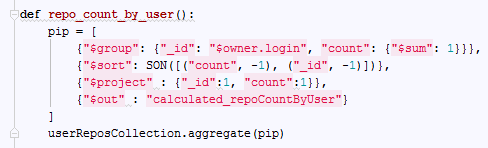
\includegraphics{Images/pymongo-aggregation.PNG}
%}
%\caption{Sample Python code which pulls the total repository count per user using PyMongo and the MongoDB Aggregation Framework.}
%\label{fig:repo-count-code}
%\end{center}
%\end{figure}


\subsection{Original vs. Forked Projects}
\label{origvsforked}
In order to determine original versus forked projects from our collection of local RTP projects, we needed to take a look at the "fork" field for each repository. The "fork" field takes a boolean value of True or False. We wrote a Python function that would count the number of original projects per user as well as the number of forked projects per user. Two separate collections were created in our local MongoDB instance and the data was later analyzed to help us understand if local users were forking existing projects more often than creating new projects.

\section{Overall RTP Activity}
Once we had established a baseline of GitHub users and associated repositories, we could start calculating RTP users' overall activity. As discussed, one piece of this research that particularly interested us was to find out how many users were actually active open source community members, in other words, how many users are actively contributing towards live projects. For this, we wanted to ignore users that joined for one project or homework assignment, for example, and never came back again. 

In order to gain an understanding of the overall GitHub activity in RTP, we investigated from a few different angles. We first aimed to understand trends in overall activity over the lifetime of a local user account and then wanted to understand who is still currently active. We are defining "active" in this research as making a commit to a repository over the last 6 months. In order to determine overall activity, we created the following questions to guide us:

\begin{enumerate}
\item Total number of commits by owner
\item Total number of active repositories based off commits
\item Total number of forks
\item Total number of pull requests
\item Total number of stargazers
\end{enumerate}

Question 1-2 are covered in section \ref{sec-commits}. Question 3 was covered already in section \ref{origvsforked}. Question 4 is covered in section \ref{sec-pullreqs} and question 5 is in section \ref{sec-stargazing}. The results from each data collection method are captured in Chapter \ref{Chapter:Findings}.

\subsection{Collecting User Commits and Active Repositories}
\label{sec-commits}
As part of the study of overall activity within our local scope, we sought to understand what the total number of commits per project looked like. In order to collect this information, we used the meta-data located in the GHTorrent MySQL instance in combination with our already existing collection of local users in our local MongoDB instance. We queried the GHTorrent MySQL instance for the name of the repository, the owner name, the count of commits as well as the last commit date. Figure~\ref{fig:commits-per-project} shows the script in detail. Due to the massive volume of commit data, we let this script run overnight as it took several hours to complete. During the initial run, we ran into errors that were not caught in the code. MongoDB requires UTF-8 encoding and hence any entries which were not UTF-8 that we tried to insert into our local MongoDB instance failed (\textbf{Error Message: bson.errors.InvalidStringData: strings in documents must be valid UTF-8}). We altered the script to translate these field names to binary to get past this, logging any future failure details to a new collection. The subsequent run of this script did not give us any failures, however. The total number of commits per project (as well as their associated timestamps) were useful is helping us answer defined questions on RTP user activity and current participation in the open source community.

\begin{figure}
\footnotesize
\begin{lstlisting}
def commit_numbers():

    query = "select p.name, u.login, u.name,
    max(c.created_at), count(c.id) 
    from projects p, users u, commits c"\
    " where u.id = p.owner_id"\
    " and c.project_id = p.id"\
    " and u.login = %s"\
    " and p.name = %s"\
    " group by p.name, u.login, u.name"

    reposList = userReposCollection.find(
    	{},{"owner.login":1, "name":1}) 
        
    i = 0
    try:
        for x in reposList:
            if(i > 16969):
                mySqlCursor = mySqlDB.cursor()
                mySqlCursor.execute(query,(x['owner']['login'],x['name']))
                data = mySqlCursor.fetchall()
                for row in data:
                    myLocalDB.testCollection.insert([
                        {"project_name":row[0],
                        "owner_login": row[1],
                        "owner_name": bson.Binary(str(row[2])),
                        "last_commit_date": row[3],
                        "commit_count":row[4]}])
                    print "done with ", x['owner']['login'], x['name'], i
            i+=1
            # print x['owner']['login'], x['name']
    except Exception, e:
        myLocalDB.rejects.insert({"failed":i})
\end{lstlisting}
\caption{This Python script was used to collect the number of commits per local project.}
\label{fig:commits-per-project}
\end{figure}

%\begin{figure}
%\begin{center}
%\resizebox{\textwidth}{!}{
%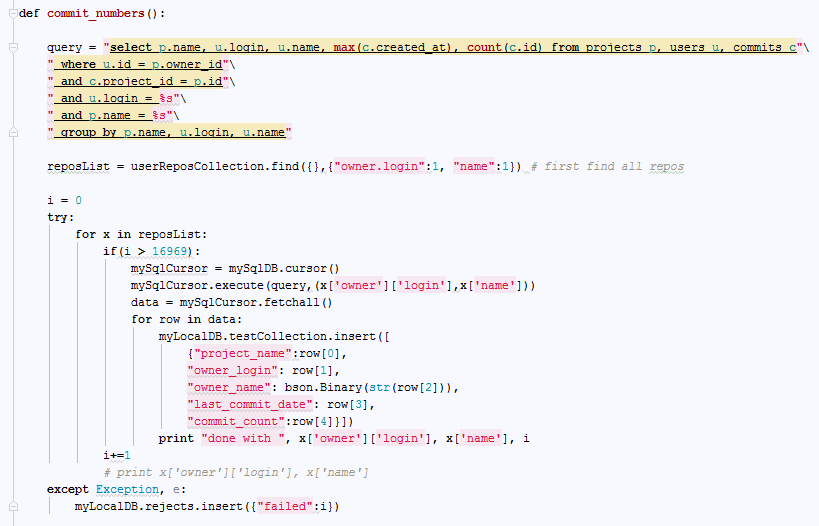
\includegraphics{Images/commitNumbers.PNG}
%}
%\caption{This Python script was used to collect the number of commits per local project.}
%\label{fig:commits-per-project}
%\end{center}
%\end{figure}

\subsection{Collecting Pull Requests}
\label{sec-pullreqs}
In order to determine overall user activity, we needed to understand how many pull requests had been submitted by each RTP user. For this, we pulled data directly out of the GHTorrent MySQL database and inserted it into our local MongoDB instance. The SQL query we used performed a union of two select statements. The first statement joins locally owned repositories on the head repository ID in the pull requests table and the second statement joins on the base repository id in the pull requests table. This is done to ensure we collect any repositories that have been forked. The script used for collecting the pull requests is shown in Figure \ref{fig:pullrequests}. 

\begin{figure}
\footnotesize
\begin{lstlisting}
def getPullReqs():

    query = "(select u.login, p.name, count(*) 
    	as 'prcount', 'head' as 'repotype'"\
            " from projects p, users u, pull_requests pr"\
            " where p.owner_id = u.id"\
            " and pr.head_repo_id = p.id"\
            " and p.deleted is false"\
            " and p.forked_from is null"\
            " and u.login = %s"\
            " group by p.id"\
            " order by count(*) desc)"\
            " UNION"\
            " (select u.login, p.name, count(*) 
            	as 'prcount', 'base' as 'repotype'"\
            " from projects p, users u, pull_requests pr"\
            " where p.owner_id = u.id"\
            " and pr.base_repo_id = p.id"\
            " and p.deleted is false"\
            " and p.forked_from is null"\
            " and u.login = %s"\
            " group by p.id"\
            " order by count(*) desc)"

    myUsers = githubRTPUsers.find({},{"login":1}) # first find all usernames

    i = 0
    try:
        for x in myUsers:
            mySqlCursor = mySqlDB.cursor()
            mySqlCursor.execute(query,(x['login'],x['login']))
            data = mySqlCursor.fetchall()
            for row in data:
                myLocalDB.calculated_pullReqByUser.insert([
                    {"login":row[0],
                    "name": row[1],
                    "prcount": row[2],
                    "repotype": row[3]}])
                print "done with ", x['login'], i
            i+=1
    except Exception, e:
        print e
        myLocalDB.rejects.insert({"failed":i})
\end{lstlisting}
\caption{Python script used to query for pull requests from the GHTorrent MySQL database and then insert them into our local MongoDB instance.}
\label{fig:pullrequests}
\end{figure}

\section{Social Networking - "Stargazing"}
\label{sec-stargazing}
In addition to overall open source activity, we were interested in understanding the popularity of local users and their work. One way to do this was to look into how many users had repositories which were being "starred" or "followed". We wrote a Python script to query the GHTorrent MongoDB instance (watchers collection), using our collected list of RTP users and their owned repositories. We inserted the results from this script into a new collection in our local MongoDB instance. Figure~\ref{fig:stargazers} shows an example of what one of these entries looks like. 

After the list of "stargazers" had been collected, we again used the MongoDB aggregation framework to find out which local repositories were the most popular.  Figure~\ref{fig:stargazers-count} shows what this query looked like. One thing to note for this collection is that if a user is a “contributor” on a project then the stars for that project end up in our list - some examples of this are shown in Chapter~\ref{Chapter:Findings} (Data Findings). Lastly, we utilized aggregation to find out how many followers each local user had (see Figure~\ref{fig:stargazing-aggregation}).

\begin{figure}
\tiny
\begin{lstlisting}
> db.githubRTPStargazers.findOne()
{
        "_id" : ObjectId("539eb518bd35432a2004564c"),
        "following_url" : "https://api.github.com/users/HagamosVideojuegos/following{/other_user}",
        "events_url" : "https://api.github.com/users/HagamosVideojuegos/events{/privacy}",
        "organizations_url" : "https://api.github.com/users/HagamosVideojuegos/orgs",
        "url" : "https://api.github.com/users/HagamosVideojuegos",
        "gists_url" : "https://api.github.com/users/HagamosVideojuegos/gists{/gist_id}",
        "html_url" : "https://github.com/HagamosVideojuegos",
        "subscriptions_url" : "https://api.github.com/users/HagamosVideojuegos/subscriptions",
        "repo" : "BombaFiesta-Unity3D-Futile",
        "owner" : "edbartley",
        "avatar_url" : "https://avatars.githubusercontent.com/u/6969130?",
        "repos_url" : "https://api.github.com/users/HagamosVideojuegos/repos",
        "received_events_url" : "https://api.github.com/users/HagamosVideojuegos/received_events",
        "gravatar_id" : "028308b2ed248bbd76fa686f0855006e",
        "starred_url" : "https://api.github.com/users/HagamosVideojuegos/starred{/owner}{/repo}",
        "site_admin" : false,
        "login" : "HagamosVideojuegos",
        "type" : "User",
        "id" : 6969130,
        "followers_url" : "https://api.github.com/users/HagamosVideojuegos/followers"
}
\end{lstlisting}
\caption{A view into the stargazers collection.}
\label{fig:stargazers}
\end{figure}

%\begin{figure}
%\begin{center}
%\resizebox{\textwidth}{!}{
%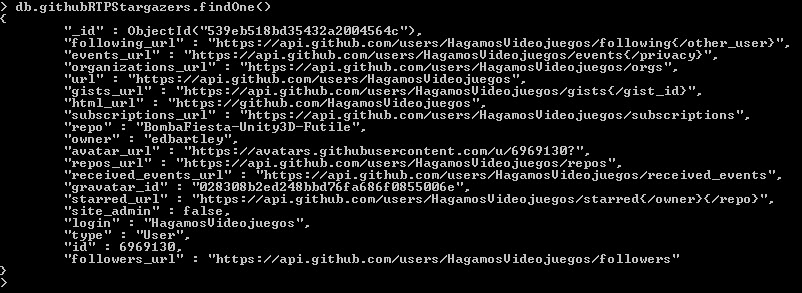
\includegraphics{Images/RTPStargazers_findOne.jpg}
%}
%\caption{A view into the stargazers collection.} 
%\label{fig:stargazers}
%\end{center}
%\end{figure}

\begin{figure}
\begin{lstlisting}
db.githubRTPStargazers.aggregate(
[
	{$group: {
    	_id:"$repo", 
        total: {$sum: 1}}},{$sort:{total:-1}
   	}
])
\end{lstlisting}
\caption{Aggregation used to find out how many followers each local repository contained.}
\label{fig:stargazers-count}
\end{figure}

\begin{figure}
\begin{lstlisting}
def stargazing():
    pip = [
        {"$group": {"_id": "$owner", "count": {"$sum": 1}}},
        {"$sort": SON([("count", -1), ("_id", -1)])},
        {"$project" : {"_id":1, "count":1, "owner":1,"repo":1}},
        {"$out" : "calculated_totalStargazers"}
    ]
    stargazersCollection.aggregate(pip)
\end{lstlisting}
\caption{Python script used to calculate the number of followers that each RTP user has.}
\label{fig:stargazing-aggregation}
\end{figure}

%\begin{figure}
%\begin{center}
%\resizebox{\textwidth}{!}{
%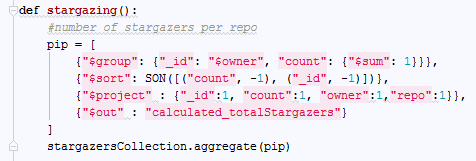
\includegraphics{Images/Stargazing-Aggregation.PNG}
%}
%\caption{Python script used to calculate the number of followers that each RTP user has.\label{fig:stargazing-aggregation}} 
%\end{center}
%\end{figure}

% % !TEX root = main.tex
\chapter{Data Findings}
\label{Chapter:Findings}

Once the data collection method was developed and implemented, we started mining through the information collected in an attempt to answer the key questions described in chapter \ref{Chapter:Introduction} for the RTP region. We broke down those high level questions into more specific items described in section \ref{key-res-questions}. To find out about GitHub users in the RTP region, we provide answers to questions one through five. In order to see what the overall numbers look like in terms of projects developed out of the RTP area as well as their associated activity and current relevance, we answer questions six through twelve. Finally, in order to gain a better understanding of how RTP users are taking advantage of GitHub social networking features, as well as their overall popularity, we answer questions thirteen through fifteen.

We found that the easiest way to illustrate a lot of these findings was to create visual representations of the data collected. For this, we used Plot.ly, an open source framework for developing data visualizations in various languages \cite{_plotly_????}. Figure~\ref{fig:user-count-by-city-code} shows an example of the creation of a bar chart using this framework. The remainder of this chapter is broken down into specific sections dedicated to answering the key research questions. We first go into an overview of RTP users, then drill into RTP specific repositories, overall open source contribution activity and lastly look into the usage of social networking features available on GitHub.

\section{Key Research Questions}
\label{key-res-questions}
\begin{enumerate}
\item How many users does the RTP area have overall?
\item How many users does the RTP area have by type (User vs. Organization)?
\item What is the average number of repositories per user in RTP (overall)?
\item How long have local users been GitHub members? How many users have been around since GitHub started?
\item What city has the most users?
\item What is the repository count by User? 
\item What is the repository count by Organization?
\item Who has the most repositories overall in the RTP area?
\item Are users creating original repositories or forking existing repositories or collaborating more often?
\item What do the commit numbers look like for local RTP repositories?
\item How many of the RTP repositories are active (for this research, active is defined as repositories which contain changes that have been committed at some point over the last 6 months)?
\item What is the average life of a local project?
\item Are many local users being "followed"?
\item Are local repositories being starred often?
\item What are the most popular programming languages?
\end{enumerate}

\begin{figure}
\footnotesize
\begin{lstlisting}
def userCountByCity_BarChart():
    results = userCountByCity.find({"count":{"$gte" : 20}})

    x = []
    y = []

    for i in results:
        x.append(i['_id'])
        y.append(i['count'])

    plotly.offline.plot({
    "data": [
        Bar(x=x, y=y,
            marker=dict(
            color='rgb(158,202,225)',
            line=dict(
                color='rgb(8,48,107)',
                width=1.5
            ),
        ),
        opacity=0.6)
    ],
    "layout": Layout(
        title="Number Of Users By City (User Count Greater Than 20)",
        annotations=[
        dict(
            x=xi,
            y=yi,
            text=str(yi),
            xanchor='center',
            yanchor='bottom',
            showarrow=False,
        ) for xi, yi in zip(x, y)]
    )
    })
\end{lstlisting}
\normalsize
\caption{Sample Python code which pulls the total repository count per user using PyMongo and the Aggregation Framework.}
\label{fig:user-count-by-city-code}
\end{figure}

%\begin{figure}
%\begin{center}
%\resizebox{\textwidth}{!}{
%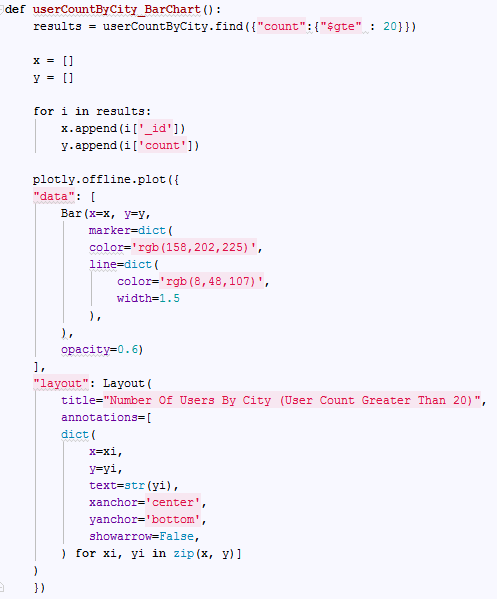
\includegraphics{Images/userCountByCity-pymongo.PNG}
%}
%\caption{Sample Python code which pulls the total repository count per user using PyMongo and the Aggregation Framework.} 
%\label{fig:user-count-by-city-code}
%\end{center}
%\end{figure}

%questions 1-5
\section{Users Overview}
In this section, we will focus on answering questions one through five from section \ref{key-res-questions}. We will find out how many users the RTP area has overall, by both User and Organization type. We will also find out how many repositories each user has on average, how long they have been members and which city in the region has the most users. The collection of RTP users was the most important dataset in this research as everything else was built upon them. As discussed in chapter \ref{Chapter:RTP}, RTP is a very prominent location for the information technology industry as a whole. We suspected we would find open source activity in the area but did not have any baselines from other locations to compare to. We managed to find 3,234 total RTP users (again, only being able to find users that had their location listed on GitHub). This means only .1\% of the RTP population (as also discussed in chapter 2, there are 3 million people living in a 60 mile radius of the park) are members of GitHub. Of these, 47 percent of them were located in Raleigh. Figure \ref{fig-userCountByCityBarChart} shows a bar chart created with Plot.ly with the number of RTP users by city. This chart only shows 8 cities as we filtered out all cities that had less than 20 users. Out of the 90 cities identified through NCLM (see \ref{fig:rtp-cities}), only 33 contained users contributing on GitHub. Raleigh, Durham and Chapel Hill had the highest number of users in the area which is understandable given these locations are home to the major research universities as well as many of the large technology companies referenced in chapter \ref{Chapter:RTP}. We also looked into the total number of RTP users by user type, finding that the majority of accounts were "User" - 2,982 with the remaining 252 being of type "Organization".

\begin{figure}
\begin{center}
\resizebox{\textwidth}{!}{
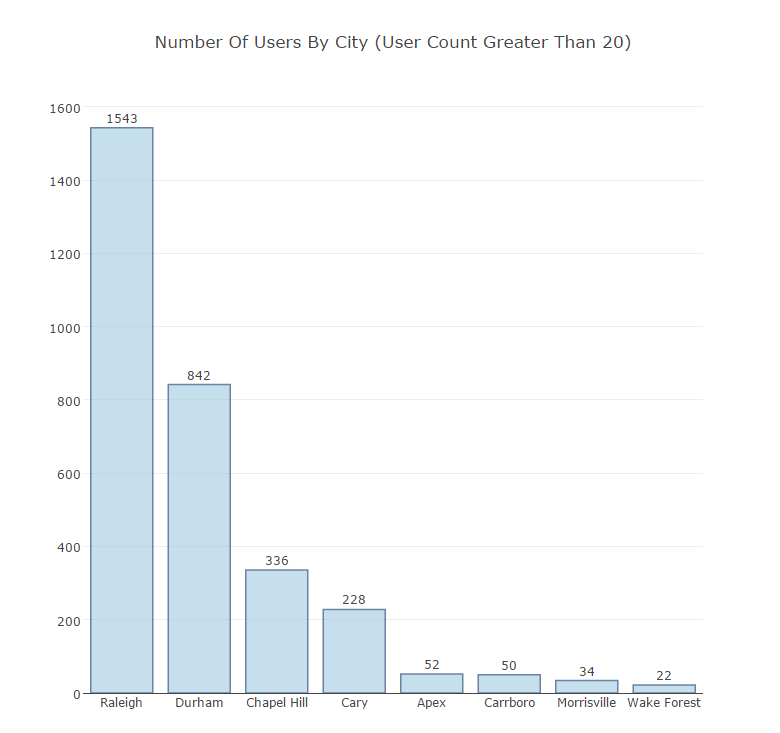
\includegraphics{Charts/userCountByCity-final.PNG}
}
\caption{This figure shows all RTP cities that have more than 20 users.} 
\label{fig-userCountByCityBarChart}
\end{center}
\end{figure}

Another metric that we were interested in gathering was how long the local RTP users had been members on GitHub. As mentioned in the previous chapter, GitHub has been around for 8 years now. We were curious to find out how many local users had created their accounts when the service went live. There ended up being around 130 users that have had their accounts for 7-8 years. Out of these accounts, 61\% (80 users) have been active (or submitted a commit) over the last 6 months. Figure \ref{fig-activeUsers} shows the script used to determine active users who have been members on GitHub for over 7 years. It was interesting to note that over half of the oldest users were still active on GitHub.

%\begin{figure}
%\label{fig-activeUsers}
%\begin{center}
%\resizebox{\textwidth}{!}{
%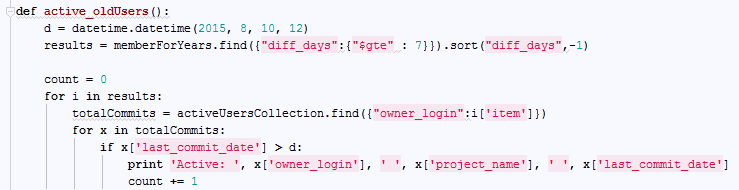
\includegraphics[width=16cm]{Images/active_legacyUsers.PNG}
%}
%\caption{This figure shows the Python script used to find RTP users that have been members on GitHub for more than 7 years and are still active today.} 
%\end{center}
%\end{figure}

\begin{figure}
\footnotesize
\begin{lstlisting}
def active_oldUsers():
  d = datetime.datetime(2015, 8, 10, 12)
  results = memberForYears.find({"diff_days":{"$gte" : 7}})
                          .sort("diff_days",-1)

  count = 0
  for i in results:
    totalCommits = activeUsersCollection.find({"owner_login":i['item']})
    for x in totalCommits:
        if x['last_commit_date'] > d:
            print 'Active: ', x['owner_login'], ' ', 
                              x['project_name'], ' ',
                              x['last_commit_date']
            count += 1
\end{lstlisting}
\caption{This figure shows the Python script used to find RTP users that have been members on GitHub for more than 7 years and are still active today.}
\label{fig-activeUsers}
\end{figure}

% questions 6-8
\section{Repositories Overview}
\label{sec:RepositoriesOverview}
In this section, we will present an overview of the RTP repositories found during the data collection phase through answering questions six through nine from section \ref{key-res-questions}. We will learn how many repositories have been created out of RTP (overall and by user type), as well as which RTP user has the most repositories. In total, we were able to find 34,825 total RTP user repositories. Of these, 31,843 were owned by a "User" type, while 2,982 were owned by an "Organization" type. There was a large amount of information available about each one of these repositories. Each repository contained an entry in a collection within our local MongoDB instance. These entries specified a number of items, including the owner details, the number of forks, whether or not the repository was a fork itself, the programming language used, the number of watchers, the create date, last updated date, as well as several API URLs that could be used to perform a number of actions on GitHub (view comment, view issues, view events, download the repository, etc.).

We calculated that RTP users have created an average of 12 repositories. The user with the most repositories had created 351, while there were a large number of users that had only created one repository. Figure \ref{fig-repoCountByUser-highest} is a chart created to show the users with the most repositories (breaking it down to users with more than 120 owned repositories). This does not necessarily mean they are active repositories and in fact could have been created and only used as a means of storage and never opened up for collaboration nor as a source code repository. The user with the most number of repositories was created as an "Organization", the account is still active today but not all 351 repositories are currently being contributed to. We will assess the activity of all repositories in section \ref{sec-ActivityOverview}. 

\begin{figure}
\resizebox{\textwidth}{!}{
\begin{bchart}[max=351]
\bcbar[text=pixbit,
 color=blue!20]{351}
\bcbar[text=jmxpearson, color=blue!20]{223}
\bcbar[text=battlemidget, color=blue!20]{193}
\bcbar[text=BanzaiMan, color=blue!20]{192}
\bcbar[text=apsaltis, color=blue!20]{155}
\bcbar[text=Rleahy22, color=blue!20]{151}
\bcbar[text=connyay, color=blue!20]{139}
\bcbar[text=vbatts, color=blue!20]{131}
\bcbar[text=pmuellr, color=blue!20]{131}
\bcbar[text=thewtex, color=blue!20]{129}
\bcbar[text=jcfr, color=blue!20]{127}
\bcbar[text=ryanfb, color=blue!20]{121}
\bcxlabel{Repository Count By User}
 \end{bchart}
}
\caption{This bar chart shows users with the most overall repositories in the RTP region.}
\label{fig-repoCountByUser-highest}
\end{figure}
             
The next piece of information gathered about overall repositories in the RTP region was the total number of original versus forked projects. We were interested in understanding if users created original projects more often than forking from already existing projects. Table \ref{fig-forked-repos} and \ref{fig-orig-repos} show the findings from these calculations. After sampling this data, we found out that around 40\% of the projects in RTP are forked and 59\% are original. This does not exclude inactive repositories. What this tells us is that while more than half of the repositories are original projects created by the RTP owner, there are still a large number of projects that have been forked from already existing projects with a possible intent to collaborate.

\begin{table}
\parbox{.45\linewidth}{
\centering
\begin{tabular}{|c|c|}
\hline
Forked Repositories & Total Users\\
\hline
15,244 & 2099\\
\hline
\end{tabular}
\caption{Total Original Repositories in RTP}
\label{fig-forked-repos}
}
\hfill
\parbox{.45\linewidth}{
\centering
\begin{tabular}{|c|c|}
\hline
Original Repositories & Total Users\\
\hline
19,745 & 2518\\
\hline
\end{tabular}
\caption{Total Forked Repositories in RTP}
\label{fig-orig-repos}
}
\end{table}

% 10-11
\section{Activity Overview}
\label{sec-ActivityOverview}
We did some investigating into how many local users were active while seeking to answer questions ten and eleven. We find out what the commit numbers look like for RTP repositories, as well as the overall activity of RTP users. As discussed previously, we defined a user as being "active" if they  have made a commit sometime over the last 6 months. We found that 2,559 unique users had made a commit over the last 6 months on GitHub which we seemed quite high. We can't necessarily say that 79\% of RTP users are active on GitHub, however, due to the fact that was discussed in chapter \ref{Chapter:Background}, when committing a change in GitHub, the author field is free text in many cases. We can see this quite clearly in the collected dataset on commits. There are unfortunately many users who lazily entered data such as their first name only (i.e. "Ben") instead of their full name, e-mail address or login name as an identifier. As part of future research, it would be useful to programatically attempt to match authors to their rightful GitHub account, similar to what the GHTorrent project does (as discussed already in section \ref{sec-GHTorrentProject}). This way we would be able to calculate a more accurate number on the total number of active users in the area.

We were able to say for certain that there are 6,756 unique RTP owned repositories that are active on GitHub, since this field cannot be free text. This means that of all the repositories owned by RTP users, 19\% of them are active. Figure \ref{fig-projCommits6mon} shows all users with more than 2,000 commits over the last 6 months. We looked a bit further into the top 10 active users (by login ID) to find out more information about them. All 10 of these users have made more than 2,000 commits to projects over the last 6 months (see Table \ref{table-top10activeusers}). As we can see, 70\% of these users are set up as Organizations on GitHub, which makes sense in that there would be more commits than "User" projects where there may be only one contributor. It was hard to identify a specific trend between these numbers. For example, these project owners either heavily utilize pull requests, or they don't. This observation could be explained by the fact that users and organizations utilize different workflows as already discussed in section \ref{sec-GitHub}.


\begin{figure}
%\resizebox{\textwidth}{!}{
\begin{bchart}[max=11.312,width=.9\textwidth]
\bcbar[text=OpenNMS, color=blue!20, value=11312]{11.312}
\bcbar[text=tee3, color=blue!20, value=3665]{3.665}
\bcbar[text=bredelings, color=blue!20, value=3145]{3.145}
\bcbar[text=duke-libraries, color=blue!20, value=2809]{2.809}
\bcbar[text=mautic, color=blue!20, value=2788]{2.788}
\bcbar[text=caktus, color=blue!20, value=2738]{2.738}
\bcbar[text=automatak, color=blue!20, value=2684]{2.684}
\bcbar[text=waldenraines, color=blue!20, value=2407]{2.407}
\bcbar[text=pencilblue, color=blue!20, value=2357]{2.357}
\bcbar[text=UNC-Libraries, color=blue!20, value=2234]{2.234}
\bcbar[text=jhinkey, color=blue!20, value=2149]{2.149}
\bcbar[text=deads2k, color=blue!20, value=2077]{2.077}
\bcxlabel{Total Commits per User}
 \end{bchart}
%}
\caption{This figure shows all users with more than 1000 commits over the last 6 months.}
\label{fig-projCommits6mon}
\end{figure}


\begin{table}
\centering
\resizebox{\textwidth}{!}{
\begin{tabular}{|c|c|c|c|c|c|c|}
\hline
User ID & User Type & Member Since & City & \# Projects & \# Pull Reqs & \# Stargazers \\
\hline
OpenNMS & Organization & Dec-12 & Pittsboro & 66 & 864 & 254 \\
\hline
tee3 & User & Mar-10 & Raleigh & 18 & 2 & 5 \\
\hline
bredelings & User & Oct-09 & Durham & 8 & 2 & 15 \\
\hline
duke-libraries & Organization & Oct-12 & Durham & 52 & 2310 & 40 \\
\hline
mautic & Organization & Aug-13 & Raleigh & 14 & 718 & 479 \\
\hline
caktus & Organization & Apr-10 & Durham & 89 & 1602 & 856 \\
\hline
automatak & Organization & Jan-13 & Raleigh & 10 & 42 & 81\\
\hline
waldenraines & User & Apr-13 & Raleigh & 17 & 0 & 0 \\ 
\hline
pencilblue & Organization & Feb-14 & Raleigh & 15 & 751 & 1257 \\
\hline
UNC-Libraries & Organization & Jan-11 & Chapel Hill & 28 & 766 & 157 \\
\hline
\end{tabular}
}
\caption{More information on the top 10 active RTP users (have pushed commits in the last 6 months). This chart shows their total number of projects, pull requests and stargazers. }
\label{table-top10activeusers}
\end{table} 

%12-14
\section{Popularity Overview}
\label{sec-PopularityOverview}
Finally, after reviewing metrics on RTP users, their repositories and overall activity on GitHub, we decided to take a look into the data to find out how "popular" our local users and projects were. In this section, we will discuss questions twelve through fifteen. We will seek to find out if many RTP users are being "followed" or "starred". We will also find out what the most popular programming language is. As mentioned in chapter \ref{Chapter:Background}, GitHub gives us an easy way to do this with their built in social media features such as "stargazing". We were able to dig into the collected data to find out that some of our users are actually somewhat popular. 1,253 users (39\%) contain at least one follower. We have 2 local users that have more than 10,000 followers. Figure \ref{fig-stargazersByUser} gives us a view of the number of stargazers that each user has (where the total number of followers is greater than 1000). The RTP user with the most stargazers is an author of a book on PHP, who lives and works in Chapel Hill.

\begin{figure}
%\resizebox{\textwidth}{!}{
\begin{bchart}[max=125.71,width=.9\textwidth]
\bcbar[text=codeguy, color=blue!20, value=12571]{125.71}
\bcbar[text=fogleman, color=blue!20, value=11682]{120.82}
\bcbar[text=jlong, color=blue!20, value=7856]{80.56}
\bcbar[text=alebcay, color=blue!20, value=6249]{70.49}
\bcbar[text=twotoasters, color=blue!20, value=3798]{60.98}
\bcbar[text=cognitect, color=blue!20, value=2586]{55.86}
\bcbar[text=smashingboxes, color=blue!20, value=2428]{50.28}
\bcbar[text=jaymedavis, color=blue!20, value=1564]{45.64}
\bcbar[text=clojure-cookbook, color=blue!20, value=1554]{40.54}
\bcbar[text=alandipert, color=blue!20, value=1553]{39.53}
\bcbar[text=mapier, color=blue!20, value=1304]{35.04}
\bcbar[text=pencilblue, color=blue!20, value=1257]{33.57}
\bcbar[text=kconner, color=blue!20, value=1204]{31.04}
\bcbar[text=stuarthalloway, color=blue!20, value=1187]{29.87}
\bcbar[text=bwsewell, color=blue!20, value=1145]{27.45}
\bcbar[text=yfactorial, color=blue!20, value=1073]{24.073}
\bcxlabel{Total Stargazers per User}
 \end{bchart}
%}
\caption{This figure shows the number of followers that each user has (where the count of followers is greater than 1000).}
\label{fig-stargazersByUser}
\end{figure}

Another metric we collected was the overall programming language popularity in this region. We aggregated the repository collections and counted the number of occurrences for each language, ignoring any projects that did not have the programming language listed (8,459 or 24\% did not have one listed). Figure \ref{fig-progLangPopularity} shows the number of projects that use each language in a bar chart where usage count is greater than 1,000, with JavaScript leading the way. We note that this information is what comes back from GitHub, it is important to remember that many projects will likely have more than one associated programming language.

\begin{figure}
%\resizebox{\textwidth}{!}{
\begin{bchart}[max=5.467,width=.9\textwidth]
\bcbar[text=JavaScript, color=blue!20, value=5467]{5.467}
\bcbar[text=Ruby, color=blue!20, value=4527]{4.527}
\bcbar[text=Python, color=blue!20, value=3457]{3.457}
\bcbar[text=Java, color=blue!20, value=2062]{2.062}
\bcbar[text=CSS, color=blue!20, value=1349]{1.349}
\bcbar[text=PHP, color=blue!20, value=1255]{1.255}
\bcbar[text=Shell, color=blue!20, value=1069]{1.069}
\bcxlabel{Top GitHub Programming Languages in RTP}
 \end{bchart}
%}
\caption{This figure shows the most popular programming languages in the RTP region, where the usage count is greater than 1000.}
\label{fig-progLangPopularity}
\end{figure}


%15
\section{Average Life of a RTP Project}
\label{sec-lifeOfAProj}
One of the additional data points that we decided to collect was what the average life of a GitHub project owned by a user in RTP looked like (question fifteen). We found out that the oldest RTP repository was created less than a month after GitHub was founded, "depth-charge". Figure \ref{fig-mongoqueryOldestRTPRepo} shows the query used to find this information in our local MongoDB database. This particular repository was created 8 years ago and hasn't been updated since.

\begin{figure}
\label{fig-mongoqueryOldestRTPRepo}
\begin{lstlisting}
> db.githubRTPUsersRepos
	.find({},
    	{"owner.login":1,"created_at":"1","name":1})
    .sort({"created_at":1})
    .limit(1)
> { 
	"_id" : ObjectId("52bedd67bd3543677400823a"), 
	"owner" : { "login" : "bscofield" }, 
    	"name" : "depth-charge", 
    	"created_at" : ISODate("2008-02-27T12:42:10Z") 
  }
\end{lstlisting}
\caption{Finding the oldest RTP repository from MongoDB's shell  (query and result).}
\end{figure}

Finally, we also found that the average life of a RTP project is 102 days. This was calculated by subtracting the created date from the last commit date and then averaging the entire gathered list. We found that the shortest project was 1 day and that there are plenty of projects that are still ongoing and active.

\section{Threats to Validity}
Due to the quality of data that we were able to retrieve for this project, there are several threats to validity that must be mentioned. As already discussed, it is important to remember that the location field in GitHub is not required, hence there is likely a large population of users that are left out of our research because they haven't given a location or have possibly given an inaccurate one. This was a limitation with our research due to the fact that we were heavily interested in querying for users that lived in such a specific location. Additionally, it was difficult for us to find out the exact number of commits per user. This is because users are able to enter free text into the authors field when committing a change in the GitHub shell (command line). This impacted the results from the mining for overall activity in the RTP region. We looked into pulling data from other sources to supplement the information from GitHub. An example source being LinkedIn, which was unsuccessful due to restrictions with the licensing of their REST API.

% % !TEX root = main.tex
\chapter{Conclusion}
\label{Chapter:Conclusion}

The purpose of this research was to shed light on the open source activities in the Research Triangle Park region using information mined from  GitHub. We began the data collection phase by gathering metrics around how many people in the RTP area were involved in open source projects (from both personal and organizational levels). This information was then used to explore repositories developed out of the RTP area, looking into characteristics such as the programming languages used, their associated activity, and current relevance of the various projects. Lastly, we explored how RTP users were involved in the social media aspects of GitHub. In summary, we found that, as a whole, the RTP region is not heavily involved in the open source community, but we were able to identify a number of users that were prominent on the platform both from the single user and organizational perspective.

As part of future research, it would be interesting to extend these experiments to cover other locations with a similar technology industry profile, providing additional context for the current results and providing insight into how open source development differs in different parts of the United States and in technology hubs in other countries. It would also be interesting to add a temporal aspect to this research, exploring how open source development activities change over time. Teams and individual developers could also use this work to find out which cities have the most users, repositories, open source activity, and overall popularity, potentially by providing this data through a portal. Lastly, it would also be interesting to compare findings such as the most popular programming languages to the job requirements in the local markets to see if any trends can be identified. The scripts developed for this thesis, used as part of the data collection and analysis phases, are themselves available on GitHub under an open-source license.

% % \restoregeometry


% %%---------------------------------------------------------------------------%%
% %%  Bibliography 

% %--
% % \begin{spacing}{1}
% %  \setlength\bibitemsep{11pt} %22pt = 2*11pt, where fontsize is 11pt
% %  \addcontentsline{toc}{chapter}{{\uppercase{\bibname}}} 
% % %{\chaptertitlename\ \thechapter}{11pt}{\bf\filcenter}
% % \titlespacing*{\chapter}{0pt}{-0.5in-9pt}{22pt}
% % \renewcommand{\bibsetup}{\thispagestyle{empty}}
% % \printbibliography[heading=myheading]
% % \end{spacing}



% % %%---------------------------------------------------------------------------%%
% % % Appendices
% % \restoregeometry
% % \appendix
% % %\renewcommand\thechapter{}
% % %\renewcommand\thesection{\arabic{section}}

% % \newgeometry{margin=1in,lmargin=1.25in,footskip=\chapterfootskip, includehead, includefoot}


% % %\include{Appendix-A/Appendix-A}

% % \restoregeometry

% %%---------------------------------------------------------------------------%%
% \backmatter


% \end{document}